% ========================================================================
% Appendix: Quasiparticle generation, population, and trapping in NbN
%           transmons operating at 4 K
%
% Style: Watson-Crick understatement, calibrated hedging.
% Include-ready version: assumes preamble in main.tex provides
% amsmath, amssymb, physics, siunitx, graphicx, hyperref, cleveref.
%
% To include, add to main.tex inside \appendix block:
%   % ========================================================================
% Appendix: Quasiparticle generation, population, and trapping in NbN
%           transmons operating at 4 K
%
% Style: Watson-Crick understatement, calibrated hedging.
% Include-ready version: assumes preamble in main.tex provides
% amsmath, amssymb, physics, siunitx, graphicx, hyperref, cleveref.
%
% To include, add to main.tex inside \appendix block:
%   % ========================================================================
% Appendix: Quasiparticle generation, population, and trapping in NbN
%           transmons operating at 4 K
%
% Style: Watson-Crick understatement, calibrated hedging.
% Include-ready version: assumes preamble in main.tex provides
% amsmath, amssymb, physics, siunitx, graphicx, hyperref, cleveref.
%
% To include, add to main.tex inside \appendix block:
%   % ========================================================================
% Appendix: Quasiparticle generation, population, and trapping in NbN
%           transmons operating at 4 K
%
% Style: Watson-Crick understatement, calibrated hedging.
% Include-ready version: assumes preamble in main.tex provides
% amsmath, amssymb, physics, siunitx, graphicx, hyperref, cleveref.
%
% To include, add to main.tex inside \appendix block:
%   \include{chapters/appendix_quasiparticles}
%
% Cross-references defined here (so quantum_algorithms.tex can \cref them):
%   \label{app:qp}, \label{app:qp:kinetic}, \label{app:qp:traps},
%   \label{app:qp:eq:nss-full}, \label{app:qp:eq:s-min}
% ========================================================================

\chapter[Quasiparticle generation, population, and trapping]%
        {Quasiparticle generation, population, and trapping\\
         in superconducting transmons at \SI{4}{\kelvin}}
\label{app:qp}

% Custom commands - only define if not already in main preamble
\providecommand{\xqp}{x_{\rm qp}}
\providecommand{\xqpth}{x_{\rm qp}^{\rm th}}
\providecommand{\kBb}{k_{\rm B}}
\providecommand{\Eone}{E_{J1}}
\providecommand{\Etwo}{E_{J2}}

\section{Bogoliubov quasiparticles and Fermi--Dirac statistics}
\label{app:qp:bogoliubov}

The elementary excitations of a BCS superconductor are not Cooper pairs but
\emph{Bogoliubov quasiparticles}, coherent superpositions of an electron and a
hole created by
\begin{equation}
  \gamma^\dagger_{k\sigma}
   \;=\; u_k\, c^\dagger_{k\sigma} \;-\; \sigma v_k\, c_{-k,-\sigma}\,,
  \label{app:qp:eq:bogoliubov}
\end{equation}
with coherence factors satisfying $u_k^2 + v_k^2 = 1$.  The associated
dispersion is
\begin{equation}
  E_k \;=\; \sqrt{\xi_k^2 + \Delta^2}\,,\qquad E_k \geq \Delta\,,
  \label{app:qp:eq:bcs-dispersion}
\end{equation}
where $\xi_k$ is the normal-state energy measured from the Fermi level and
$\Delta$ is the superconducting gap.  Because these excitations inherit the
anticommutation relations of the underlying fermionic operators, they obey
Fermi--Dirac statistics rather than Bose--Einstein.  The phonons of the
crystal lattice are bosonic, but the dissipation channel that limits qubit
coherence---tunneling of single quasiparticles through the Josephson
junction---is purely fermionic.

This distinction has two practical consequences.  First, the excitation
spectrum is gapped: producing a quasiparticle costs at least $\Delta$, so the
thermal population is exponentially suppressed.  Second, the BCS density of
states diverges at the gap edge,
\begin{equation}
  N_S(E)
  \;=\; N(0)\,\frac{|E|}{\sqrt{E^2-\Delta^2}}\,,
  \qquad |E| \geq \Delta\,,
  \label{app:qp:eq:bcs-dos}
\end{equation}
amplifying the contribution of low-energy quasiparticles which dominate
tunneling. Both features are visible in
Fig.~\ref{app:qp:fig:generation-population}.


\section{Generation and thermal population}
\label{app:qp:generation}

A phonon with energy $\hbar\omega \geq 2\Delta$ breaks a Cooper pair and
generates two quasiparticles at the gap edge,
$\gamma_e\,(E=+\Delta)$ and $\gamma_h\,(E=-\Delta)$
(Fig.~\ref{app:qp:fig:generation-population}a).  Detailed balance with the
phonon bath fixes the equilibrium density.  Folding
Eq.~\eqref{app:qp:eq:bcs-dos} with the Fermi--Dirac distribution and
integrating, in the limit $\kBb T \ll \Delta$ one obtains
\begin{equation}
  \boxed{\;
    \xqpth(T)
    \;\equiv\; \frac{n_{\rm qp}}{n_{\rm cp}}
    \;\simeq\; \sqrt{\frac{2\pi \kBb T}{\Delta}}\,\exp\!\left(-\frac{\Delta}{\kBb T}\right)\,,
  \;}
  \label{app:qp:eq:xqp-thermal}
\end{equation}
where $n_{\rm cp} = 2N(0)\Delta$ is the Cooper-pair density.  For NbN at the
target operating temperature $T = \SI{4}{\kelvin}$, with
$\Delta \simeq \SI{2.8}{\milli\electronvolt}$, we obtain
$\xqpth(\SI{4}{\kelvin}) \simeq 2.7 \times 10^{-4}$.  This number is the
\emph{thermal floor}: any non-equilibrium contribution decreases the steady
state below this value only if a removal mechanism with rate exceeding the
phonon-driven generation is provided.

\begin{figure}[t]
  \centering
  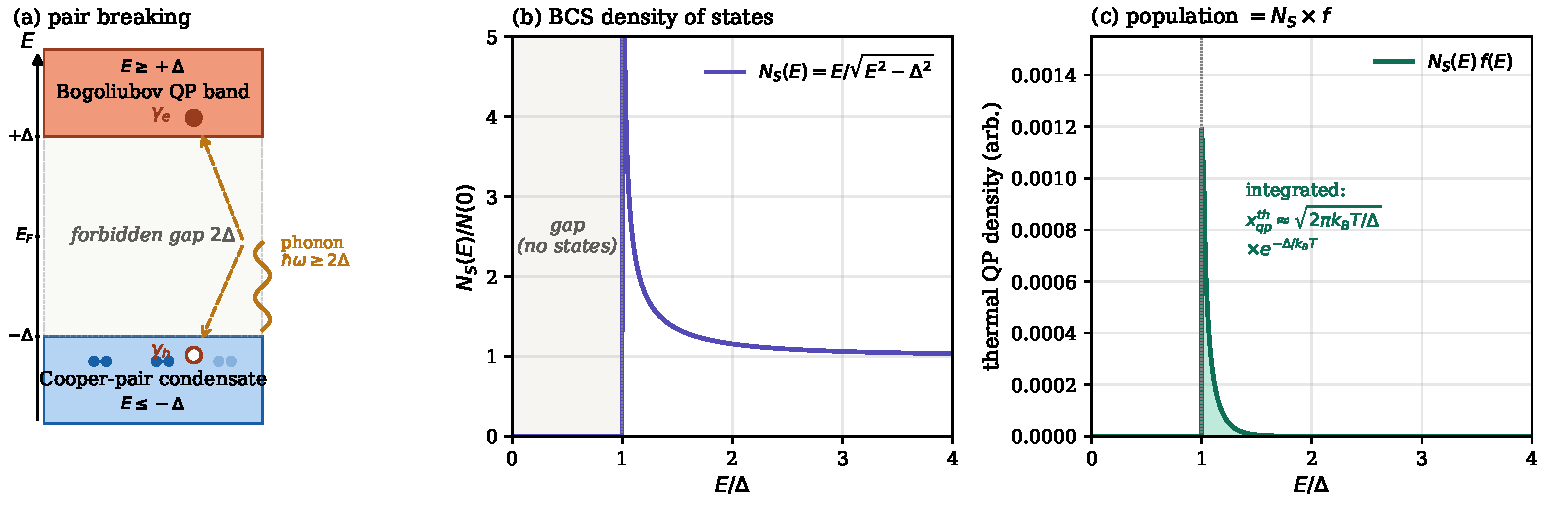
\includegraphics[width=\textwidth]{chapters/qh_figures/fig_qp_generation_population.pdf}
  \caption{Quasiparticle physics in three panels.
    (a)~A phonon with $\hbar\omega \geq 2\Delta$ breaks a Cooper pair,
    producing an electron-like quasiparticle $\gamma_e$ at $E=+\Delta$ and a
    hole-like quasiparticle $\gamma_h$ at $E=-\Delta$.
    (b)~The BCS density of states (Eq.~\ref{app:qp:eq:bcs-dos}) diverges at
    $|E| = \Delta$.
    (c)~The thermal population $N_S(E)\,f(E)$ is concentrated within a
    few $\kBb T$ of the gap edge; the integrated density is given by
    Eq.~\ref{app:qp:eq:xqp-thermal}.}
  \label{app:qp:fig:generation-population}
\end{figure}


\section{Kinetic equations: Rothwarf--Taylor with traps}
\label{app:qp:kinetic}

The dynamics of the integrated quasiparticle density $n$ and of the population
$N$ of pair-breaking phonons ($\hbar\omega = 2\Delta$) follow the
Rothwarf--Taylor equations~\cite{Rothwarf1967}, here augmented by an
empirical trap rate $s$ acting on quasiparticles:
\begin{align}
  \dot n &= I_{qp} \;+\; 2\beta N \;-\; R\,n^2 \;-\; s\,n\,,
  \label{app:qp:eq:RT-n}\\[2pt]
  \dot N &= I_{ph} \;-\; \beta N \;+\; \tfrac{1}{2} R\,n^2
            \;-\; \gamma_{\rm esc}\,(N - N_{\rm eq})\,.
  \label{app:qp:eq:RT-N}
\end{align}
$R$ is the bimolecular recombination coefficient
($R = 2/(n_{\rm cp}\,\tau_R^{\rm eq})$, with $\tau_R$ from
Kaplan~\cite{Kaplan1976}); $\beta$ the pair-breaking coefficient;
$\gamma_{\rm esc}$ the rate at which $2\Delta$ phonons escape to the
substrate; $I_{qp}, I_{ph}$ external sources.  Eliminating $N$ in the steady
state and defining the effective recombination rate
$R_{\rm eff} = R\,\gamma_{\rm esc}/(\beta + \gamma_{\rm esc})$, the
quasiparticle equation reduces to
\begin{equation}
  \dot n
  \;=\; G \;-\; s\,n \;-\; R_{\rm eff}\,n^2\,,
  \label{app:qp:eq:reduced-kinetic}
\end{equation}
with $G$ a total effective generation rate fixed by detailed balance
($G = R_{\rm eff}\,n_{\rm eq}^2$ in the absence of external sources).
Equation~\eqref{app:qp:eq:reduced-kinetic} is a Riccati equation and admits
closed-form analytical solutions in three regimes.

\subsection{Regime~1: pure relaxation, no generation, no trap}

For $G=s=0$ and initial condition $n(0)=n_0$, the equation
$\dot n = -R\,n^2$ separates and integrates to
\begin{equation}
  n(t) \;=\; \frac{n_0}{1 + R\,n_0\, t}\,.
  \label{app:qp:eq:hyperbolic-decay}
\end{equation}
The decay is \emph{hyperbolic}, not exponential. This is the signature of
bimolecular recombination: two quasiparticles are required to form a Cooper
pair, so the rate scales as $n^2$. This $1/t$ behaviour is observed in
pump-probe experiments on MgB$_2$ and Pb~\cite{Demsar2003}.

\subsection{Regime~2: trap-dominated linear decay}

When $s\,n \gg R\,n^2$ (sufficiently low density or sufficiently large $s$),
Eq.~\eqref{app:qp:eq:reduced-kinetic} linearises to $\dot n = G - s\,n$,
yielding
\begin{equation}
  n(t) \;=\; n^{\rm ss} \;+\; (n_0 - n^{\rm ss})\,e^{-s\,t}\,,
  \qquad n^{\rm ss} \;=\; \frac{G}{s}\,.
  \label{app:qp:eq:trap-linear}
\end{equation}
The decay is exponential, with time constant $\tau_{\rm tr} = 1/s$. This is
the regime in which normal-metal traps operate in transmon
qubits~\cite{Riwar2016}.

\subsection{Regime~3: full Riccati solution}

The general steady-state solution is obtained from the positive root of
$G - s n - R n^2 = 0$:
\begin{equation}
  \boxed{\;
    n^{\rm ss}
    \;=\; \frac{-\,s \;+\; \sqrt{s^2 + 4 R G}}{2 R}\,.
  \;}
  \label{app:qp:eq:nss-full}
\end{equation}
The crossover between the recombination-dominated and the trap-dominated
regime occurs at $s^* = 2\sqrt{R G}$: for $s \ll s^*$,
Eq.~\eqref{app:qp:eq:nss-full} reduces to $\sqrt{G/R}$
(recombination-limited); for $s \gg s^*$ it reduces to $G/s$
(trap-limited). The full time-dependent solution can be written in closed
form by separating variables; the relaxation rate towards the steady state
is $\Gamma_{\rm relax} = \sqrt{s^2 + 4 R G}$. The three regimes are
summarised in Fig.~\ref{app:qp:fig:kinetic-regimes} and compared with
direct numerical integration of Eq.~\eqref{app:qp:eq:reduced-kinetic}.

\begin{figure}[t]
  \centering
  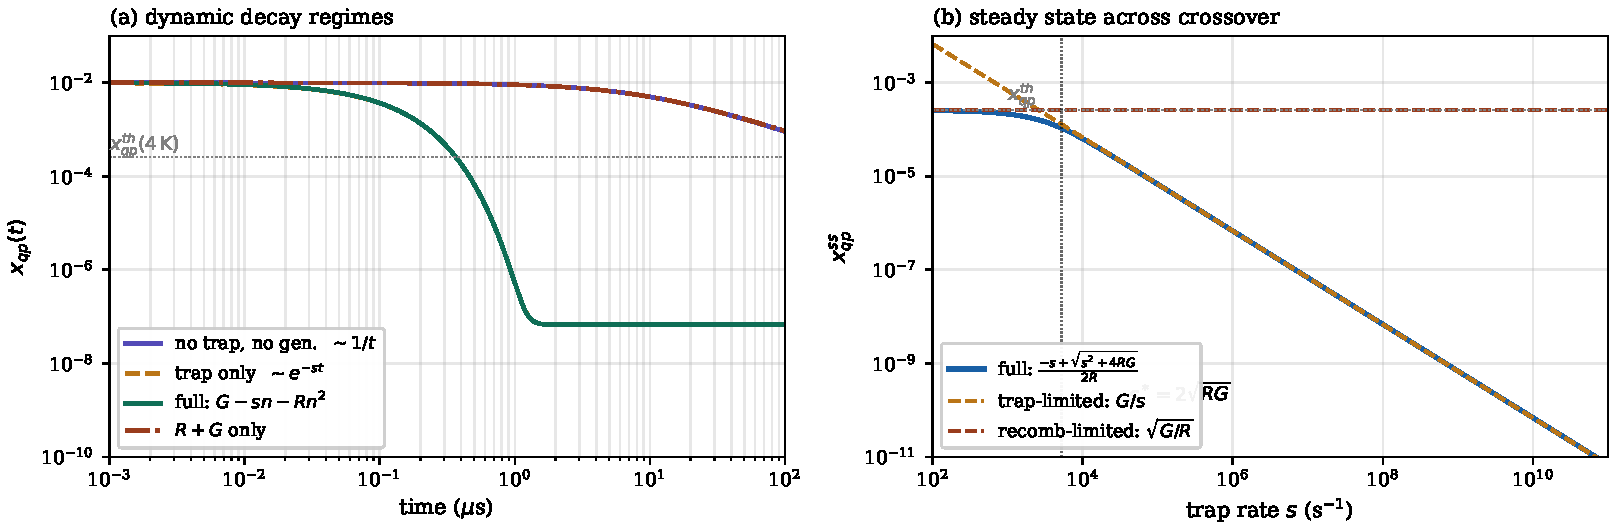
\includegraphics[width=\textwidth]{chapters/qh_figures/fig_kinetic_regimes.pdf}
  \caption{Analytical solutions of the reduced kinetic
    equation~\eqref{app:qp:eq:reduced-kinetic}, verified against numerical
    ODE integration. (a)~Dynamic decay from a pulse injection
    $n_0 = 10^{-2}$ for the three limiting cases. (b)~Steady-state
    density as a function of the trap rate $s$, showing the crossover at
    $s^* = 2\sqrt{R G}$ between recombination-limited ($\sqrt{G/R}$) and
    trap-limited ($G/s$) behaviour. Parameters: $R = 10^7\,{\rm s}^{-1}$
    (NbN benchmark), $G = R\,(\xqpth)^2$ at \SI{4}{\kelvin}.}
  \label{app:qp:fig:kinetic-regimes}
\end{figure}


\section{Implications for an NbN transmon at \SI{4}{\kelvin}}
\label{app:qp:implications}

The intrinsic quasiparticle-induced relaxation rate for a transmon is given,
in the small-$\hbar\omega/\Delta$ limit, by~\cite{Catelani2011}
\begin{equation}
  \frac{1}{T_1^{\rm qp}}
  \;=\; \frac{\omega_{01}}{\pi}\,\xqp\,
        \sqrt{\frac{2\Delta}{\hbar\omega_{01}}}\,.
  \label{app:qp:eq:T1qp}
\end{equation}
For NbN at \SI{4}{\kelvin}, with $\Delta = \SI{2.8}{\milli\electronvolt}$
and $\omega_{01}/2\pi = \SI{5}{\giga\hertz}$, substituting
$\xqp = \xqpth = 2.7\times 10^{-4}$ gives
\begin{equation}
  T_1^{\rm qp,\,intrinsic} \;\simeq\; \SI{20}{\nano\second}\,.
  \label{app:qp:eq:T1-intrinsic}
\end{equation}
Reaching a coherence time of $T_1 = \SI{49}{\micro\second}$, compatible with
the gate fidelities required by the algorithms discussed in
Chapter~\ref{chap:algorithms}, therefore requires reducing $\xqp$ below its
thermal-equilibrium value by approximately three orders of magnitude. Two
engineering approaches are conceivable: \emph{gap engineering}, which
exponentially suppresses one of the two tunneling channels across an
asymmetric junction, and \emph{trap engineering}, which lowers $\xqp$ in the
steady state of the kinetic balance. We examine both, and conclude that
only the latter is effective in the thermal regime.


\section{Why gap engineering does not work at \SI{4}{\kelvin}}
\label{app:qp:gap-fails}

In an asymmetric Josephson junction with electrode gaps $\Delta_1 > \Delta_2$,
Marchegiani \emph{et al.}~\cite{Marchegiani2022} have shown that quasiparticle
tunneling from the low-gap electrode is suppressed by a factor
$\exp[-(\Delta_1 - \Delta_2)/\kBb T]$ \emph{provided the quasiparticles are
out of thermal equilibrium}.  In that regime the population on the low-gap
side is fixed externally, and the suppression genuinely reduces the rate.
At \SI{4}{\kelvin}, however, both sides of the junction are in thermal
equilibrium with the phonon bath, and the population on the low-gap side
satisfies $\xqp^{\rm th}(\Delta_2) \gg \xqp^{\rm th}(\Delta_1)$.  The two
contributions to the total tunneling rate read
\begin{align}
  \Gamma_{1\to 2}
   &\;\propto\; \xqp^{\rm th}(\Delta_1)
   \qquad &&\text{(downhill, not suppressed)}\,,
   \label{app:qp:eq:rate-down}\\
  \Gamma_{2\to 1}
   &\;\propto\; \xqp^{\rm th}(\Delta_2)\,e^{-(\Delta_1-\Delta_2)/\kBb T}
   \qquad &&\text{(uphill, suppressed)}\,.
   \label{app:qp:eq:rate-up}
\end{align}
Substituting Eq.~\eqref{app:qp:eq:xqp-thermal}, the factor
$e^{-\Delta_2/\kBb T}$ in $\xqp^{\rm th}(\Delta_2)$ cancels against the
suppression $e^{-(\Delta_1-\Delta_2)/\kBb T}$, leaving
\begin{equation}
  \Gamma_{2\to 1}
   \;\propto\; \sqrt{\Delta_1/\Delta_2}\,\,\xqp^{\rm th}(\Delta_1)\,,
\end{equation}
of the same order as $\Gamma_{1\to 2}$.  The total rate is governed by
$e^{-\Delta_{\max}/\kBb T}$, i.e.\ by the larger gap, and is essentially
independent of the gap asymmetry.  Numerical evaluation with our kinetic
model confirms this: across the range of realistic candidate materials
(NbN/Nb, NbN/NbTiN, NbN/TaN), the $T_1^{\rm qp}$ at \SI{4}{\kelvin}
remains within a factor of two of the symmetric NbN/NbN baseline.
Gap engineering retains its value as a defence against cosmic-ray
quasiparticle bursts~\cite{McEwen2024} and for charge-parity
preservation~\cite{Kamenov2024}, but does not by itself relax the thermal
ceiling on $T_1^{\rm qp}$.


\section{Trap engineering: the working route}
\label{app:qp:traps}

A region of normal metal in tunnel contact with the superconductor provides
a sink for quasiparticles.  A quasiparticle that crosses the N--S barrier
relaxes inelastically to subgap energies in the normal metal, and the
superconducting gap then prevents its return
(Fig.~\ref{app:qp:fig:trap-mechanism}a).  In the diffusive regime, the
effective trap rate $s$ depends on the trap area $A_{\rm trap}$, on its
tunnel transparency $T_{\rm NS}$, on the normal-metal electron--electron
relaxation rate, and on the geometric configuration of the qubit pads:
the underlying spatial problem is one of diffusion to localised
sinks~\cite{Riwar2016,Hosseinkhani2017}.

\begin{figure}[t]
  \centering
  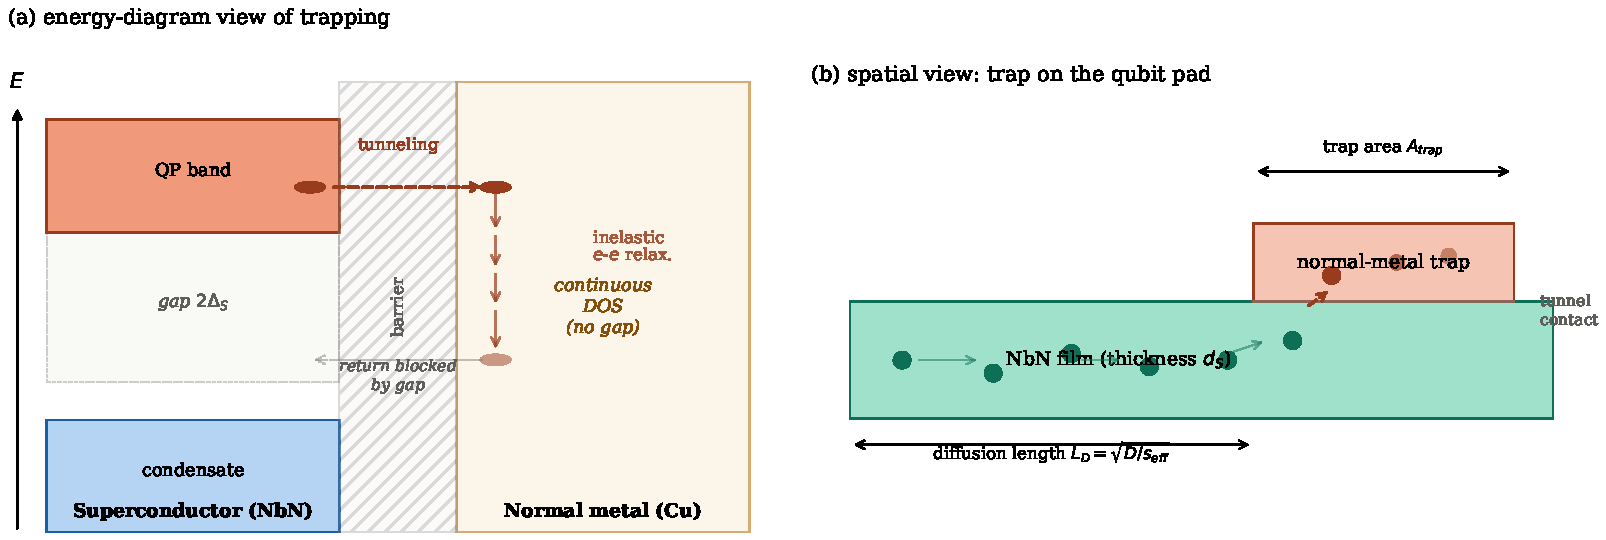
\includegraphics[width=\textwidth]{chapters/qh_figures/fig_trap_mechanism.pdf}
  \caption{Normal-metal trap mechanism.
    (a)~Energy diagram: a quasiparticle tunnels from the QP band of the
    superconductor into the continuous density of states of the normal
    metal, relaxes inelastically to subgap energies, and cannot return
    because the gap blocks the way.
    (b)~Spatial view: a quasiparticle diffusing in the NbN film with
    diffusion length $L_D = \sqrt{D/s_{\rm eff}}$ is captured by the
    normal-metal pad of area $A_{\rm trap}$ deposited in tunnel contact.}
  \label{app:qp:fig:trap-mechanism}
\end{figure}

Within Eq.~\eqref{app:qp:eq:nss-full} the requirement that
$\xqp^{\rm ss}$ falls sufficiently below the thermal floor to support
$T_1 = \SI{49}{\micro\second}$ can be expressed as a constraint on $s$.
Using Eq.~\eqref{app:qp:eq:T1qp} with the parameters of
Sec.~\ref{app:qp:implications}, the target reads
$\xqp \simeq 1.1\times 10^{-7}$.  In the trap-limited regime,
\begin{equation}
  s_{\rm min}
   \;=\; \frac{G_{\rm th}}{\xqp^{\rm target}}
   \;=\; \frac{R\,(\xqpth)^2}{\xqp^{\rm target}}
   \;\sim\; 10^{7}\,{\rm s}^{-1}\,.
  \label{app:qp:eq:s-min}
\end{equation}
This is approximately one order of magnitude above the rates demonstrated
in aluminum-based devices, where $s \sim 10^{4}$--$10^{6}$~s$^{-1}$ has
been measured~\cite{Riwar2016}. Reaching the target therefore requires
trap engineering at the upper edge of what has been experimentally
demonstrated, and constitutes the open experimental question discussed
below.

\subsection{Implementation strategy}
\label{app:qp:trap-implementation}

We propose deposition of normal-metal patches---of dimensions and material
detailed in Fig.~\ref{app:qp:fig:trap-engineering}---on the capacitor pads
of the asymmetric SQUID transmon, on both sides of the junctions
(\emph{bilateral} trap configuration).  The choice is dictated by the
analysis of Sec.~\ref{app:qp:gap-fails}: since the kinetic limit on $T_1$
is set by the sum of two tunneling channels, both of comparable magnitude
in thermal equilibrium, only suppressing $\xqp$ on \emph{both} electrodes
yields the multiplicative improvement.

The relevant design parameters are: the material of the trap
(Cu, Au, or Pd, with progressively shorter electron--electron relaxation
times), its area $A_{\rm trap}$, its thickness, and its distance $L$ from
the junction.  The effective trap rate in the diffusion-limited regime
saturates at $s_{\rm sat} \simeq D/L^2$, where $D$ is the quasiparticle
diffusion coefficient in NbN; pushing $s$ beyond $s_{\rm sat}$ is not
possible by increasing the trap area, and requires reducing $L$ or
increasing $D$ (cleaner films).

\begin{figure}[t]
  \centering
  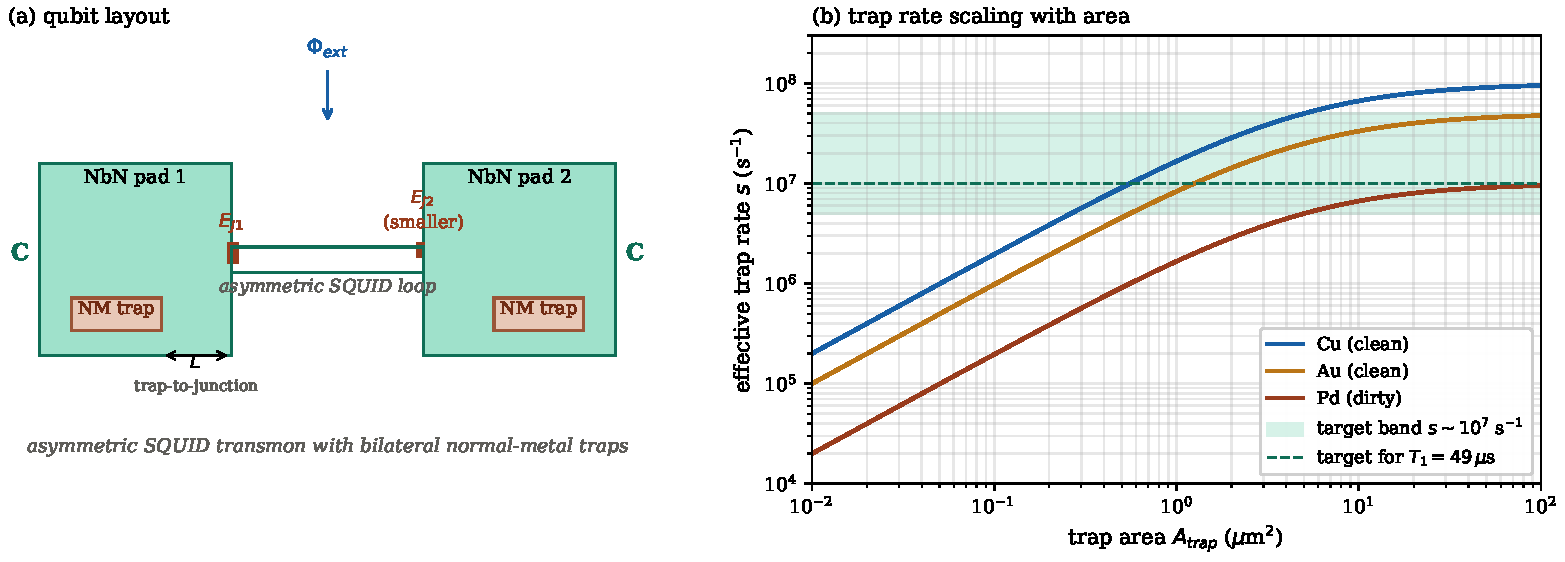
\includegraphics[width=\textwidth]{chapters/qh_figures/fig_trap_engineering.pdf}
  \caption{Trap engineering for the asymmetric SQUID transmon.
    (a)~Proposed device layout: normal-metal traps deposited on both NbN
    capacitor pads, at distance $L$ from the asymmetric SQUID. External
    flux $\Phi_{\rm ext}$ tunes the operating point between upper (USS,
    $\Phi=0$) and lower sweet spot (LSS, $\Phi=\Phi_0/2$), with the
    geometric junction asymmetry $d = (\Eone-\Etwo)/(\Eone+\Etwo)$ keeping
    $\omega_{01}$ finite at the LSS.
    (b)~Effective trap rate $s$ as a function of trap area
    $A_{\rm trap}$, for three candidate normal metals.  Saturation at
    large area reflects the diffusion-limited regime
    $s_{\rm sat} \simeq D/L^2$.  The target band $s \sim 10^{7}\,{\rm s}^{-1}$
    is required to reach $T_1 = \SI{49}{\micro\second}$ at
    \SI{4}{\kelvin}.}
  \label{app:qp:fig:trap-engineering}
\end{figure}

A trade-off exists between trap efficiency and microwave dissipation: the
normal-metal patch introduces a loss tangent that lowers the qubit quality
factor through capacitive coupling.  Locating the traps far enough from
the high-electric-field region near the junction (large $L$), while still
in the diffusion-reach of the quasiparticles, is therefore essential.
Quantitative estimation of the loss penalty requires electromagnetic
simulation of the participation ratio of the trap region, which is left
to follow-up work.


\section{Outlook}
\label{app:qp:outlook}

The analysis presented here identifies trap engineering as the only
quantitatively viable route to a microsecond-range $T_1$ in a NbN transmon
operated at \SI{4}{\kelvin}, the temperature accessible with a
two-stage pulse-tube cryocooler without sub-Kelvin refrigeration.  The
required trap rate $s \sim 10^{7}\,{\rm s}^{-1}$ sits approximately one
order of magnitude above the state of the art in aluminum-based devices
and has not been demonstrated in NbN.  The realisation of trap-engineered
NbN qubits at this performance level remains an open experimental
question, and constitutes a natural extension of the work presented in
this thesis.

%
% Cross-references defined here (so quantum_algorithms.tex can \cref them):
%   \label{app:qp}, \label{app:qp:kinetic}, \label{app:qp:traps},
%   \label{app:qp:eq:nss-full}, \label{app:qp:eq:s-min}
% ========================================================================

\chapter[Quasiparticle generation, population, and trapping]%
        {Quasiparticle generation, population, and trapping\\
         in superconducting transmons at \SI{4}{\kelvin}}
\label{app:qp}

% Custom commands - only define if not already in main preamble
\providecommand{\xqp}{x_{\rm qp}}
\providecommand{\xqpth}{x_{\rm qp}^{\rm th}}
\providecommand{\kBb}{k_{\rm B}}
\providecommand{\Eone}{E_{J1}}
\providecommand{\Etwo}{E_{J2}}

\section{Bogoliubov quasiparticles and Fermi--Dirac statistics}
\label{app:qp:bogoliubov}

The elementary excitations of a BCS superconductor are not Cooper pairs but
\emph{Bogoliubov quasiparticles}, coherent superpositions of an electron and a
hole created by
\begin{equation}
  \gamma^\dagger_{k\sigma}
   \;=\; u_k\, c^\dagger_{k\sigma} \;-\; \sigma v_k\, c_{-k,-\sigma}\,,
  \label{app:qp:eq:bogoliubov}
\end{equation}
with coherence factors satisfying $u_k^2 + v_k^2 = 1$.  The associated
dispersion is
\begin{equation}
  E_k \;=\; \sqrt{\xi_k^2 + \Delta^2}\,,\qquad E_k \geq \Delta\,,
  \label{app:qp:eq:bcs-dispersion}
\end{equation}
where $\xi_k$ is the normal-state energy measured from the Fermi level and
$\Delta$ is the superconducting gap.  Because these excitations inherit the
anticommutation relations of the underlying fermionic operators, they obey
Fermi--Dirac statistics rather than Bose--Einstein.  The phonons of the
crystal lattice are bosonic, but the dissipation channel that limits qubit
coherence---tunneling of single quasiparticles through the Josephson
junction---is purely fermionic.

This distinction has two practical consequences.  First, the excitation
spectrum is gapped: producing a quasiparticle costs at least $\Delta$, so the
thermal population is exponentially suppressed.  Second, the BCS density of
states diverges at the gap edge,
\begin{equation}
  N_S(E)
  \;=\; N(0)\,\frac{|E|}{\sqrt{E^2-\Delta^2}}\,,
  \qquad |E| \geq \Delta\,,
  \label{app:qp:eq:bcs-dos}
\end{equation}
amplifying the contribution of low-energy quasiparticles which dominate
tunneling. Both features are visible in
Fig.~\ref{app:qp:fig:generation-population}.


\section{Generation and thermal population}
\label{app:qp:generation}

A phonon with energy $\hbar\omega \geq 2\Delta$ breaks a Cooper pair and
generates two quasiparticles at the gap edge,
$\gamma_e\,(E=+\Delta)$ and $\gamma_h\,(E=-\Delta)$
(Fig.~\ref{app:qp:fig:generation-population}a).  Detailed balance with the
phonon bath fixes the equilibrium density.  Folding
Eq.~\eqref{app:qp:eq:bcs-dos} with the Fermi--Dirac distribution and
integrating, in the limit $\kBb T \ll \Delta$ one obtains
\begin{equation}
  \boxed{\;
    \xqpth(T)
    \;\equiv\; \frac{n_{\rm qp}}{n_{\rm cp}}
    \;\simeq\; \sqrt{\frac{2\pi \kBb T}{\Delta}}\,\exp\!\left(-\frac{\Delta}{\kBb T}\right)\,,
  \;}
  \label{app:qp:eq:xqp-thermal}
\end{equation}
where $n_{\rm cp} = 2N(0)\Delta$ is the Cooper-pair density.  For NbN at the
target operating temperature $T = \SI{4}{\kelvin}$, with
$\Delta \simeq \SI{2.8}{\milli\electronvolt}$, we obtain
$\xqpth(\SI{4}{\kelvin}) \simeq 2.7 \times 10^{-4}$.  This number is the
\emph{thermal floor}: any non-equilibrium contribution decreases the steady
state below this value only if a removal mechanism with rate exceeding the
phonon-driven generation is provided.

\begin{figure}[t]
  \centering
  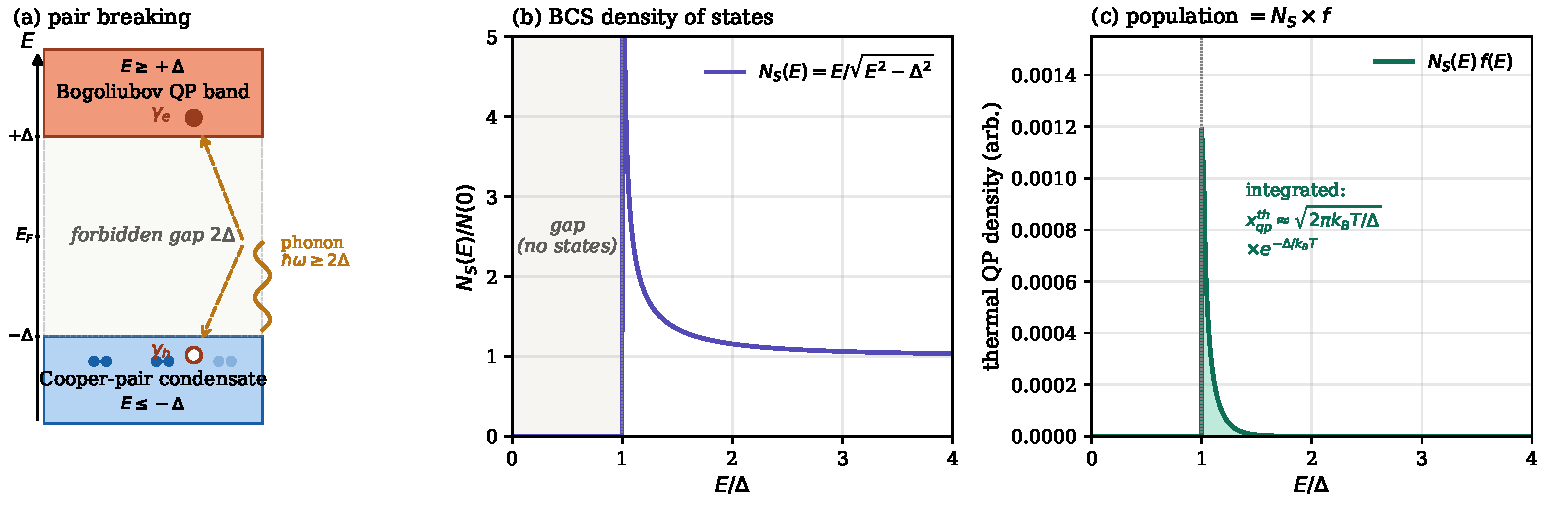
\includegraphics[width=\textwidth]{chapters/qh_figures/fig_qp_generation_population.pdf}
  \caption{Quasiparticle physics in three panels.
    (a)~A phonon with $\hbar\omega \geq 2\Delta$ breaks a Cooper pair,
    producing an electron-like quasiparticle $\gamma_e$ at $E=+\Delta$ and a
    hole-like quasiparticle $\gamma_h$ at $E=-\Delta$.
    (b)~The BCS density of states (Eq.~\ref{app:qp:eq:bcs-dos}) diverges at
    $|E| = \Delta$.
    (c)~The thermal population $N_S(E)\,f(E)$ is concentrated within a
    few $\kBb T$ of the gap edge; the integrated density is given by
    Eq.~\ref{app:qp:eq:xqp-thermal}.}
  \label{app:qp:fig:generation-population}
\end{figure}


\section{Kinetic equations: Rothwarf--Taylor with traps}
\label{app:qp:kinetic}

The dynamics of the integrated quasiparticle density $n$ and of the population
$N$ of pair-breaking phonons ($\hbar\omega = 2\Delta$) follow the
Rothwarf--Taylor equations~\cite{Rothwarf1967}, here augmented by an
empirical trap rate $s$ acting on quasiparticles:
\begin{align}
  \dot n &= I_{qp} \;+\; 2\beta N \;-\; R\,n^2 \;-\; s\,n\,,
  \label{app:qp:eq:RT-n}\\[2pt]
  \dot N &= I_{ph} \;-\; \beta N \;+\; \tfrac{1}{2} R\,n^2
            \;-\; \gamma_{\rm esc}\,(N - N_{\rm eq})\,.
  \label{app:qp:eq:RT-N}
\end{align}
$R$ is the bimolecular recombination coefficient
($R = 2/(n_{\rm cp}\,\tau_R^{\rm eq})$, with $\tau_R$ from
Kaplan~\cite{Kaplan1976}); $\beta$ the pair-breaking coefficient;
$\gamma_{\rm esc}$ the rate at which $2\Delta$ phonons escape to the
substrate; $I_{qp}, I_{ph}$ external sources.  Eliminating $N$ in the steady
state and defining the effective recombination rate
$R_{\rm eff} = R\,\gamma_{\rm esc}/(\beta + \gamma_{\rm esc})$, the
quasiparticle equation reduces to
\begin{equation}
  \dot n
  \;=\; G \;-\; s\,n \;-\; R_{\rm eff}\,n^2\,,
  \label{app:qp:eq:reduced-kinetic}
\end{equation}
with $G$ a total effective generation rate fixed by detailed balance
($G = R_{\rm eff}\,n_{\rm eq}^2$ in the absence of external sources).
Equation~\eqref{app:qp:eq:reduced-kinetic} is a Riccati equation and admits
closed-form analytical solutions in three regimes.

\subsection{Regime~1: pure relaxation, no generation, no trap}

For $G=s=0$ and initial condition $n(0)=n_0$, the equation
$\dot n = -R\,n^2$ separates and integrates to
\begin{equation}
  n(t) \;=\; \frac{n_0}{1 + R\,n_0\, t}\,.
  \label{app:qp:eq:hyperbolic-decay}
\end{equation}
The decay is \emph{hyperbolic}, not exponential. This is the signature of
bimolecular recombination: two quasiparticles are required to form a Cooper
pair, so the rate scales as $n^2$. This $1/t$ behaviour is observed in
pump-probe experiments on MgB$_2$ and Pb~\cite{Demsar2003}.

\subsection{Regime~2: trap-dominated linear decay}

When $s\,n \gg R\,n^2$ (sufficiently low density or sufficiently large $s$),
Eq.~\eqref{app:qp:eq:reduced-kinetic} linearises to $\dot n = G - s\,n$,
yielding
\begin{equation}
  n(t) \;=\; n^{\rm ss} \;+\; (n_0 - n^{\rm ss})\,e^{-s\,t}\,,
  \qquad n^{\rm ss} \;=\; \frac{G}{s}\,.
  \label{app:qp:eq:trap-linear}
\end{equation}
The decay is exponential, with time constant $\tau_{\rm tr} = 1/s$. This is
the regime in which normal-metal traps operate in transmon
qubits~\cite{Riwar2016}.

\subsection{Regime~3: full Riccati solution}

The general steady-state solution is obtained from the positive root of
$G - s n - R n^2 = 0$:
\begin{equation}
  \boxed{\;
    n^{\rm ss}
    \;=\; \frac{-\,s \;+\; \sqrt{s^2 + 4 R G}}{2 R}\,.
  \;}
  \label{app:qp:eq:nss-full}
\end{equation}
The crossover between the recombination-dominated and the trap-dominated
regime occurs at $s^* = 2\sqrt{R G}$: for $s \ll s^*$,
Eq.~\eqref{app:qp:eq:nss-full} reduces to $\sqrt{G/R}$
(recombination-limited); for $s \gg s^*$ it reduces to $G/s$
(trap-limited). The full time-dependent solution can be written in closed
form by separating variables; the relaxation rate towards the steady state
is $\Gamma_{\rm relax} = \sqrt{s^2 + 4 R G}$. The three regimes are
summarised in Fig.~\ref{app:qp:fig:kinetic-regimes} and compared with
direct numerical integration of Eq.~\eqref{app:qp:eq:reduced-kinetic}.

\begin{figure}[t]
  \centering
  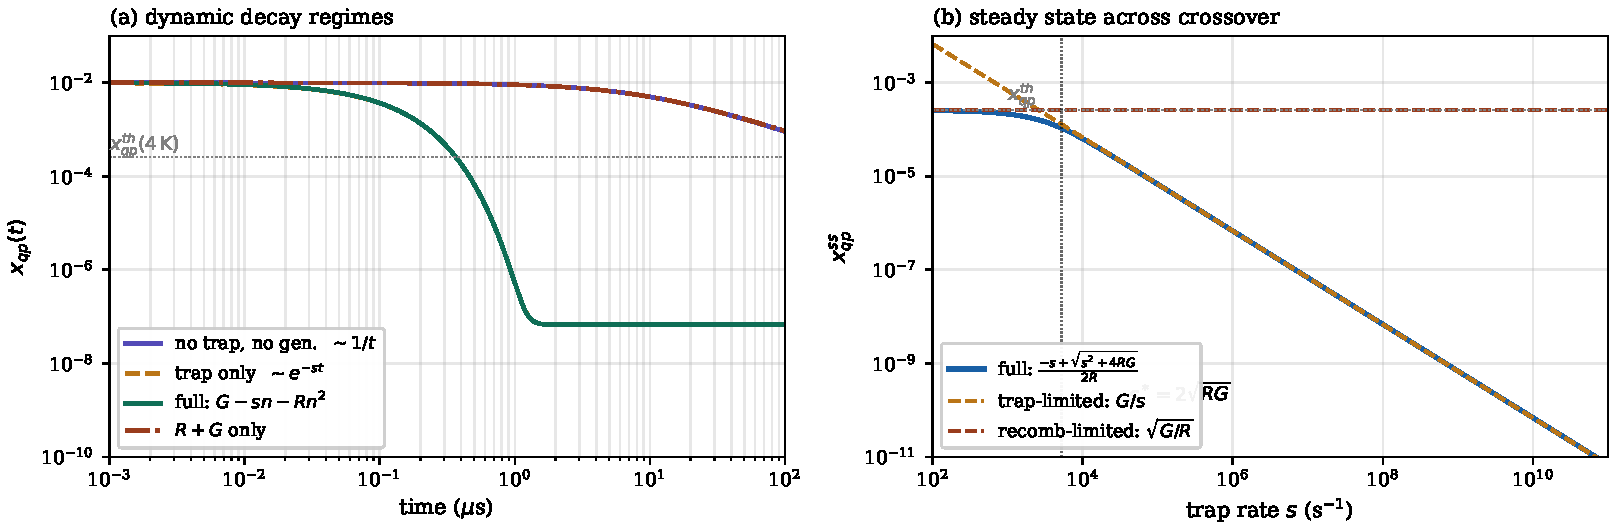
\includegraphics[width=\textwidth]{chapters/qh_figures/fig_kinetic_regimes.pdf}
  \caption{Analytical solutions of the reduced kinetic
    equation~\eqref{app:qp:eq:reduced-kinetic}, verified against numerical
    ODE integration. (a)~Dynamic decay from a pulse injection
    $n_0 = 10^{-2}$ for the three limiting cases. (b)~Steady-state
    density as a function of the trap rate $s$, showing the crossover at
    $s^* = 2\sqrt{R G}$ between recombination-limited ($\sqrt{G/R}$) and
    trap-limited ($G/s$) behaviour. Parameters: $R = 10^7\,{\rm s}^{-1}$
    (NbN benchmark), $G = R\,(\xqpth)^2$ at \SI{4}{\kelvin}.}
  \label{app:qp:fig:kinetic-regimes}
\end{figure}


\section{Implications for an NbN transmon at \SI{4}{\kelvin}}
\label{app:qp:implications}

The intrinsic quasiparticle-induced relaxation rate for a transmon is given,
in the small-$\hbar\omega/\Delta$ limit, by~\cite{Catelani2011}
\begin{equation}
  \frac{1}{T_1^{\rm qp}}
  \;=\; \frac{\omega_{01}}{\pi}\,\xqp\,
        \sqrt{\frac{2\Delta}{\hbar\omega_{01}}}\,.
  \label{app:qp:eq:T1qp}
\end{equation}
For NbN at \SI{4}{\kelvin}, with $\Delta = \SI{2.8}{\milli\electronvolt}$
and $\omega_{01}/2\pi = \SI{5}{\giga\hertz}$, substituting
$\xqp = \xqpth = 2.7\times 10^{-4}$ gives
\begin{equation}
  T_1^{\rm qp,\,intrinsic} \;\simeq\; \SI{20}{\nano\second}\,.
  \label{app:qp:eq:T1-intrinsic}
\end{equation}
Reaching a coherence time of $T_1 = \SI{49}{\micro\second}$, compatible with
the gate fidelities required by the algorithms discussed in
Chapter~\ref{chap:algorithms}, therefore requires reducing $\xqp$ below its
thermal-equilibrium value by approximately three orders of magnitude. Two
engineering approaches are conceivable: \emph{gap engineering}, which
exponentially suppresses one of the two tunneling channels across an
asymmetric junction, and \emph{trap engineering}, which lowers $\xqp$ in the
steady state of the kinetic balance. We examine both, and conclude that
only the latter is effective in the thermal regime.


\section{Why gap engineering does not work at \SI{4}{\kelvin}}
\label{app:qp:gap-fails}

In an asymmetric Josephson junction with electrode gaps $\Delta_1 > \Delta_2$,
Marchegiani \emph{et al.}~\cite{Marchegiani2022} have shown that quasiparticle
tunneling from the low-gap electrode is suppressed by a factor
$\exp[-(\Delta_1 - \Delta_2)/\kBb T]$ \emph{provided the quasiparticles are
out of thermal equilibrium}.  In that regime the population on the low-gap
side is fixed externally, and the suppression genuinely reduces the rate.
At \SI{4}{\kelvin}, however, both sides of the junction are in thermal
equilibrium with the phonon bath, and the population on the low-gap side
satisfies $\xqp^{\rm th}(\Delta_2) \gg \xqp^{\rm th}(\Delta_1)$.  The two
contributions to the total tunneling rate read
\begin{align}
  \Gamma_{1\to 2}
   &\;\propto\; \xqp^{\rm th}(\Delta_1)
   \qquad &&\text{(downhill, not suppressed)}\,,
   \label{app:qp:eq:rate-down}\\
  \Gamma_{2\to 1}
   &\;\propto\; \xqp^{\rm th}(\Delta_2)\,e^{-(\Delta_1-\Delta_2)/\kBb T}
   \qquad &&\text{(uphill, suppressed)}\,.
   \label{app:qp:eq:rate-up}
\end{align}
Substituting Eq.~\eqref{app:qp:eq:xqp-thermal}, the factor
$e^{-\Delta_2/\kBb T}$ in $\xqp^{\rm th}(\Delta_2)$ cancels against the
suppression $e^{-(\Delta_1-\Delta_2)/\kBb T}$, leaving
\begin{equation}
  \Gamma_{2\to 1}
   \;\propto\; \sqrt{\Delta_1/\Delta_2}\,\,\xqp^{\rm th}(\Delta_1)\,,
\end{equation}
of the same order as $\Gamma_{1\to 2}$.  The total rate is governed by
$e^{-\Delta_{\max}/\kBb T}$, i.e.\ by the larger gap, and is essentially
independent of the gap asymmetry.  Numerical evaluation with our kinetic
model confirms this: across the range of realistic candidate materials
(NbN/Nb, NbN/NbTiN, NbN/TaN), the $T_1^{\rm qp}$ at \SI{4}{\kelvin}
remains within a factor of two of the symmetric NbN/NbN baseline.
Gap engineering retains its value as a defence against cosmic-ray
quasiparticle bursts~\cite{McEwen2024} and for charge-parity
preservation~\cite{Kamenov2024}, but does not by itself relax the thermal
ceiling on $T_1^{\rm qp}$.


\section{Trap engineering: the working route}
\label{app:qp:traps}

A region of normal metal in tunnel contact with the superconductor provides
a sink for quasiparticles.  A quasiparticle that crosses the N--S barrier
relaxes inelastically to subgap energies in the normal metal, and the
superconducting gap then prevents its return
(Fig.~\ref{app:qp:fig:trap-mechanism}a).  In the diffusive regime, the
effective trap rate $s$ depends on the trap area $A_{\rm trap}$, on its
tunnel transparency $T_{\rm NS}$, on the normal-metal electron--electron
relaxation rate, and on the geometric configuration of the qubit pads:
the underlying spatial problem is one of diffusion to localised
sinks~\cite{Riwar2016,Hosseinkhani2017}.

\begin{figure}[t]
  \centering
  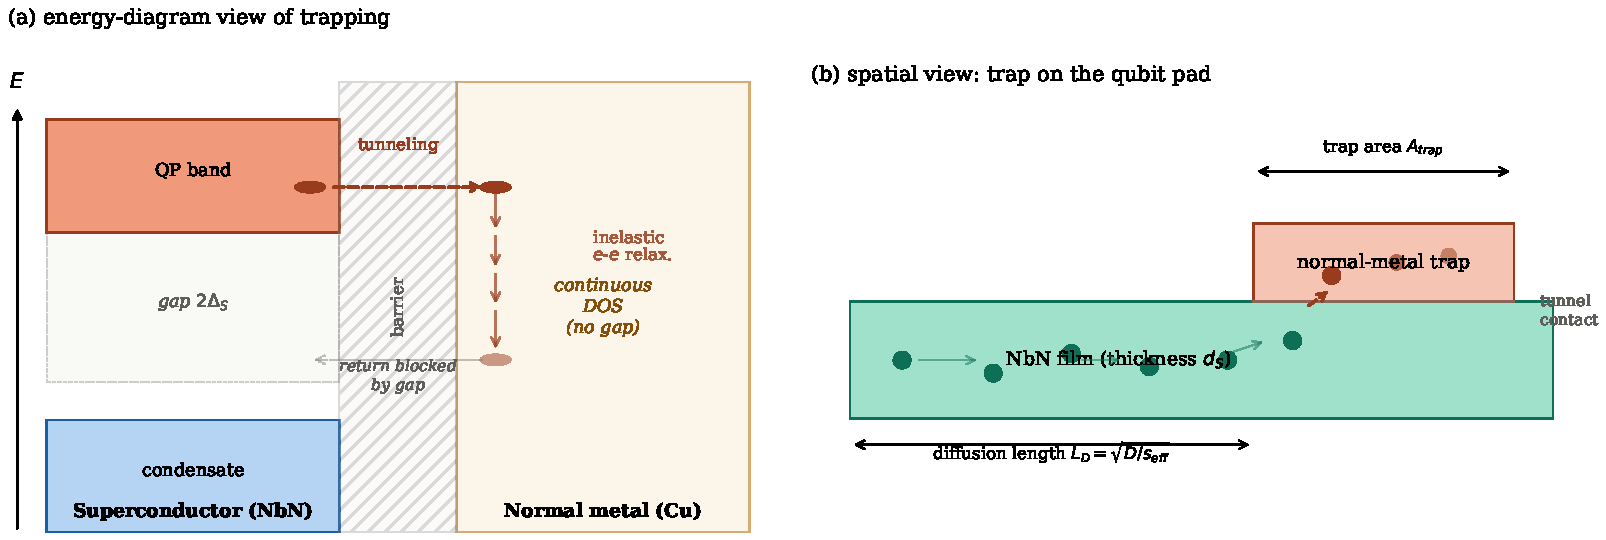
\includegraphics[width=\textwidth]{chapters/qh_figures/fig_trap_mechanism.pdf}
  \caption{Normal-metal trap mechanism.
    (a)~Energy diagram: a quasiparticle tunnels from the QP band of the
    superconductor into the continuous density of states of the normal
    metal, relaxes inelastically to subgap energies, and cannot return
    because the gap blocks the way.
    (b)~Spatial view: a quasiparticle diffusing in the NbN film with
    diffusion length $L_D = \sqrt{D/s_{\rm eff}}$ is captured by the
    normal-metal pad of area $A_{\rm trap}$ deposited in tunnel contact.}
  \label{app:qp:fig:trap-mechanism}
\end{figure}

Within Eq.~\eqref{app:qp:eq:nss-full} the requirement that
$\xqp^{\rm ss}$ falls sufficiently below the thermal floor to support
$T_1 = \SI{49}{\micro\second}$ can be expressed as a constraint on $s$.
Using Eq.~\eqref{app:qp:eq:T1qp} with the parameters of
Sec.~\ref{app:qp:implications}, the target reads
$\xqp \simeq 1.1\times 10^{-7}$.  In the trap-limited regime,
\begin{equation}
  s_{\rm min}
   \;=\; \frac{G_{\rm th}}{\xqp^{\rm target}}
   \;=\; \frac{R\,(\xqpth)^2}{\xqp^{\rm target}}
   \;\sim\; 10^{7}\,{\rm s}^{-1}\,.
  \label{app:qp:eq:s-min}
\end{equation}
This is approximately one order of magnitude above the rates demonstrated
in aluminum-based devices, where $s \sim 10^{4}$--$10^{6}$~s$^{-1}$ has
been measured~\cite{Riwar2016}. Reaching the target therefore requires
trap engineering at the upper edge of what has been experimentally
demonstrated, and constitutes the open experimental question discussed
below.

\subsection{Implementation strategy}
\label{app:qp:trap-implementation}

We propose deposition of normal-metal patches---of dimensions and material
detailed in Fig.~\ref{app:qp:fig:trap-engineering}---on the capacitor pads
of the asymmetric SQUID transmon, on both sides of the junctions
(\emph{bilateral} trap configuration).  The choice is dictated by the
analysis of Sec.~\ref{app:qp:gap-fails}: since the kinetic limit on $T_1$
is set by the sum of two tunneling channels, both of comparable magnitude
in thermal equilibrium, only suppressing $\xqp$ on \emph{both} electrodes
yields the multiplicative improvement.

The relevant design parameters are: the material of the trap
(Cu, Au, or Pd, with progressively shorter electron--electron relaxation
times), its area $A_{\rm trap}$, its thickness, and its distance $L$ from
the junction.  The effective trap rate in the diffusion-limited regime
saturates at $s_{\rm sat} \simeq D/L^2$, where $D$ is the quasiparticle
diffusion coefficient in NbN; pushing $s$ beyond $s_{\rm sat}$ is not
possible by increasing the trap area, and requires reducing $L$ or
increasing $D$ (cleaner films).

\begin{figure}[t]
  \centering
  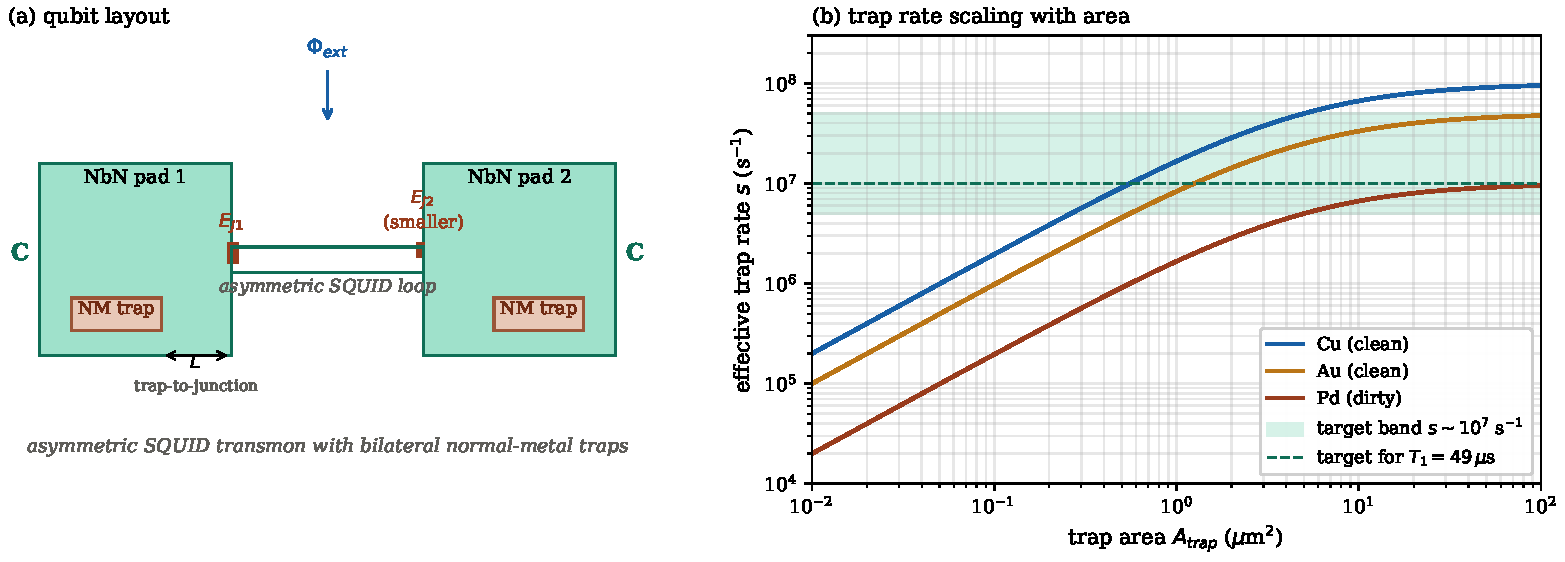
\includegraphics[width=\textwidth]{chapters/qh_figures/fig_trap_engineering.pdf}
  \caption{Trap engineering for the asymmetric SQUID transmon.
    (a)~Proposed device layout: normal-metal traps deposited on both NbN
    capacitor pads, at distance $L$ from the asymmetric SQUID. External
    flux $\Phi_{\rm ext}$ tunes the operating point between upper (USS,
    $\Phi=0$) and lower sweet spot (LSS, $\Phi=\Phi_0/2$), with the
    geometric junction asymmetry $d = (\Eone-\Etwo)/(\Eone+\Etwo)$ keeping
    $\omega_{01}$ finite at the LSS.
    (b)~Effective trap rate $s$ as a function of trap area
    $A_{\rm trap}$, for three candidate normal metals.  Saturation at
    large area reflects the diffusion-limited regime
    $s_{\rm sat} \simeq D/L^2$.  The target band $s \sim 10^{7}\,{\rm s}^{-1}$
    is required to reach $T_1 = \SI{49}{\micro\second}$ at
    \SI{4}{\kelvin}.}
  \label{app:qp:fig:trap-engineering}
\end{figure}

A trade-off exists between trap efficiency and microwave dissipation: the
normal-metal patch introduces a loss tangent that lowers the qubit quality
factor through capacitive coupling.  Locating the traps far enough from
the high-electric-field region near the junction (large $L$), while still
in the diffusion-reach of the quasiparticles, is therefore essential.
Quantitative estimation of the loss penalty requires electromagnetic
simulation of the participation ratio of the trap region, which is left
to follow-up work.


\section{Outlook}
\label{app:qp:outlook}

The analysis presented here identifies trap engineering as the only
quantitatively viable route to a microsecond-range $T_1$ in a NbN transmon
operated at \SI{4}{\kelvin}, the temperature accessible with a
two-stage pulse-tube cryocooler without sub-Kelvin refrigeration.  The
required trap rate $s \sim 10^{7}\,{\rm s}^{-1}$ sits approximately one
order of magnitude above the state of the art in aluminum-based devices
and has not been demonstrated in NbN.  The realisation of trap-engineered
NbN qubits at this performance level remains an open experimental
question, and constitutes a natural extension of the work presented in
this thesis.

%
% Cross-references defined here (so quantum_algorithms.tex can \cref them):
%   \label{app:qp}, \label{app:qp:kinetic}, \label{app:qp:traps},
%   \label{app:qp:eq:nss-full}, \label{app:qp:eq:s-min}
% ========================================================================

\chapter[Quasiparticle generation, population, and trapping]%
        {Quasiparticle generation, population, and trapping\\
         in superconducting transmons at \SI{4}{\kelvin}}
\label{app:qp}

% Custom commands - only define if not already in main preamble
\providecommand{\xqp}{x_{\rm qp}}
\providecommand{\xqpth}{x_{\rm qp}^{\rm th}}
\providecommand{\kBb}{k_{\rm B}}
\providecommand{\Eone}{E_{J1}}
\providecommand{\Etwo}{E_{J2}}

\section{Bogoliubov quasiparticles and Fermi--Dirac statistics}
\label{app:qp:bogoliubov}

The elementary excitations of a BCS superconductor are not Cooper pairs but
\emph{Bogoliubov quasiparticles}, coherent superpositions of an electron and a
hole created by
\begin{equation}
  \gamma^\dagger_{k\sigma}
   \;=\; u_k\, c^\dagger_{k\sigma} \;-\; \sigma v_k\, c_{-k,-\sigma}\,,
  \label{app:qp:eq:bogoliubov}
\end{equation}
with coherence factors satisfying $u_k^2 + v_k^2 = 1$.  The associated
dispersion is
\begin{equation}
  E_k \;=\; \sqrt{\xi_k^2 + \Delta^2}\,,\qquad E_k \geq \Delta\,,
  \label{app:qp:eq:bcs-dispersion}
\end{equation}
where $\xi_k$ is the normal-state energy measured from the Fermi level and
$\Delta$ is the superconducting gap.  Because these excitations inherit the
anticommutation relations of the underlying fermionic operators, they obey
Fermi--Dirac statistics rather than Bose--Einstein.  The phonons of the
crystal lattice are bosonic, but the dissipation channel that limits qubit
coherence---tunneling of single quasiparticles through the Josephson
junction---is purely fermionic.

This distinction has two practical consequences.  First, the excitation
spectrum is gapped: producing a quasiparticle costs at least $\Delta$, so the
thermal population is exponentially suppressed.  Second, the BCS density of
states diverges at the gap edge,
\begin{equation}
  N_S(E)
  \;=\; N(0)\,\frac{|E|}{\sqrt{E^2-\Delta^2}}\,,
  \qquad |E| \geq \Delta\,,
  \label{app:qp:eq:bcs-dos}
\end{equation}
amplifying the contribution of low-energy quasiparticles which dominate
tunneling. Both features are visible in
Fig.~\ref{app:qp:fig:generation-population}.


\section{Generation and thermal population}
\label{app:qp:generation}

A phonon with energy $\hbar\omega \geq 2\Delta$ breaks a Cooper pair and
generates two quasiparticles at the gap edge,
$\gamma_e\,(E=+\Delta)$ and $\gamma_h\,(E=-\Delta)$
(Fig.~\ref{app:qp:fig:generation-population}a).  Detailed balance with the
phonon bath fixes the equilibrium density.  Folding
Eq.~\eqref{app:qp:eq:bcs-dos} with the Fermi--Dirac distribution and
integrating, in the limit $\kBb T \ll \Delta$ one obtains
\begin{equation}
  \boxed{\;
    \xqpth(T)
    \;\equiv\; \frac{n_{\rm qp}}{n_{\rm cp}}
    \;\simeq\; \sqrt{\frac{2\pi \kBb T}{\Delta}}\,\exp\!\left(-\frac{\Delta}{\kBb T}\right)\,,
  \;}
  \label{app:qp:eq:xqp-thermal}
\end{equation}
where $n_{\rm cp} = 2N(0)\Delta$ is the Cooper-pair density.  For NbN at the
target operating temperature $T = \SI{4}{\kelvin}$, with
$\Delta \simeq \SI{2.8}{\milli\electronvolt}$, we obtain
$\xqpth(\SI{4}{\kelvin}) \simeq 2.7 \times 10^{-4}$.  This number is the
\emph{thermal floor}: any non-equilibrium contribution decreases the steady
state below this value only if a removal mechanism with rate exceeding the
phonon-driven generation is provided.

\begin{figure}[t]
  \centering
  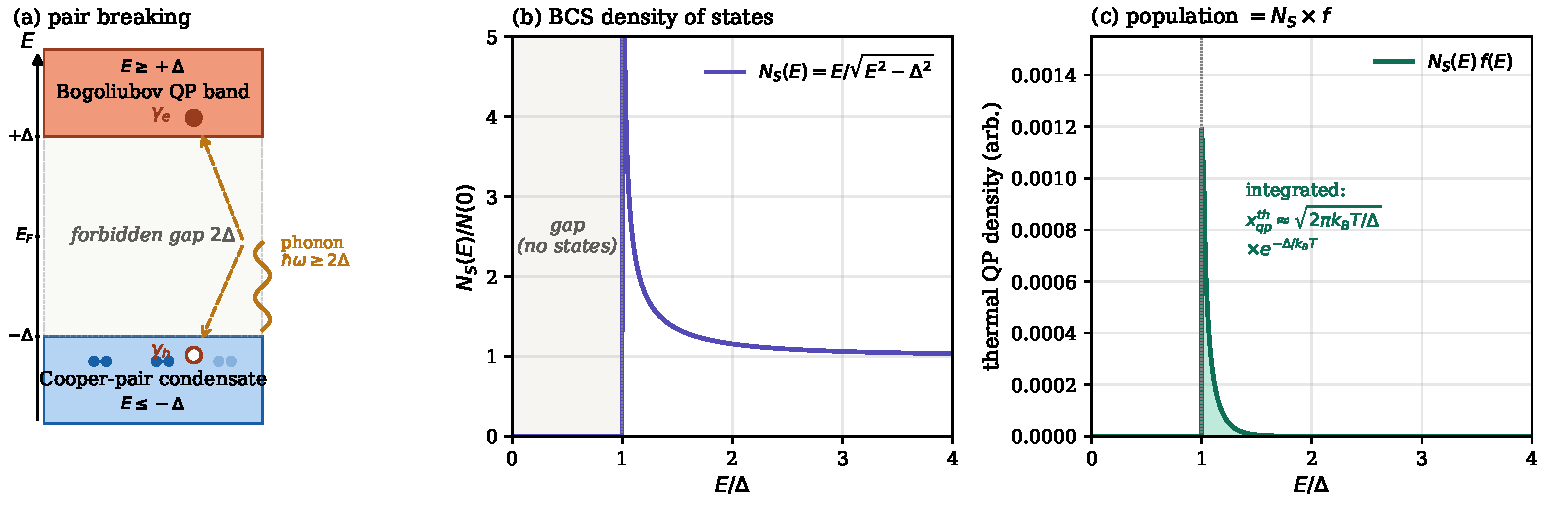
\includegraphics[width=\textwidth]{chapters/qh_figures/fig_qp_generation_population.pdf}
  \caption{Quasiparticle physics in three panels.
    (a)~A phonon with $\hbar\omega \geq 2\Delta$ breaks a Cooper pair,
    producing an electron-like quasiparticle $\gamma_e$ at $E=+\Delta$ and a
    hole-like quasiparticle $\gamma_h$ at $E=-\Delta$.
    (b)~The BCS density of states (Eq.~\ref{app:qp:eq:bcs-dos}) diverges at
    $|E| = \Delta$.
    (c)~The thermal population $N_S(E)\,f(E)$ is concentrated within a
    few $\kBb T$ of the gap edge; the integrated density is given by
    Eq.~\ref{app:qp:eq:xqp-thermal}.}
  \label{app:qp:fig:generation-population}
\end{figure}


\section{Kinetic equations: Rothwarf--Taylor with traps}
\label{app:qp:kinetic}

The dynamics of the integrated quasiparticle density $n$ and of the population
$N$ of pair-breaking phonons ($\hbar\omega = 2\Delta$) follow the
Rothwarf--Taylor equations~\cite{Rothwarf1967}, here augmented by an
empirical trap rate $s$ acting on quasiparticles:
\begin{align}
  \dot n &= I_{qp} \;+\; 2\beta N \;-\; R\,n^2 \;-\; s\,n\,,
  \label{app:qp:eq:RT-n}\\[2pt]
  \dot N &= I_{ph} \;-\; \beta N \;+\; \tfrac{1}{2} R\,n^2
            \;-\; \gamma_{\rm esc}\,(N - N_{\rm eq})\,.
  \label{app:qp:eq:RT-N}
\end{align}
$R$ is the bimolecular recombination coefficient
($R = 2/(n_{\rm cp}\,\tau_R^{\rm eq})$, with $\tau_R$ from
Kaplan~\cite{Kaplan1976}); $\beta$ the pair-breaking coefficient;
$\gamma_{\rm esc}$ the rate at which $2\Delta$ phonons escape to the
substrate; $I_{qp}, I_{ph}$ external sources.  Eliminating $N$ in the steady
state and defining the effective recombination rate
$R_{\rm eff} = R\,\gamma_{\rm esc}/(\beta + \gamma_{\rm esc})$, the
quasiparticle equation reduces to
\begin{equation}
  \dot n
  \;=\; G \;-\; s\,n \;-\; R_{\rm eff}\,n^2\,,
  \label{app:qp:eq:reduced-kinetic}
\end{equation}
with $G$ a total effective generation rate fixed by detailed balance
($G = R_{\rm eff}\,n_{\rm eq}^2$ in the absence of external sources).
Equation~\eqref{app:qp:eq:reduced-kinetic} is a Riccati equation and admits
closed-form analytical solutions in three regimes.

\subsection{Regime~1: pure relaxation, no generation, no trap}

For $G=s=0$ and initial condition $n(0)=n_0$, the equation
$\dot n = -R\,n^2$ separates and integrates to
\begin{equation}
  n(t) \;=\; \frac{n_0}{1 + R\,n_0\, t}\,.
  \label{app:qp:eq:hyperbolic-decay}
\end{equation}
The decay is \emph{hyperbolic}, not exponential. This is the signature of
bimolecular recombination: two quasiparticles are required to form a Cooper
pair, so the rate scales as $n^2$. This $1/t$ behaviour is observed in
pump-probe experiments on MgB$_2$ and Pb~\cite{Demsar2003}.

\subsection{Regime~2: trap-dominated linear decay}

When $s\,n \gg R\,n^2$ (sufficiently low density or sufficiently large $s$),
Eq.~\eqref{app:qp:eq:reduced-kinetic} linearises to $\dot n = G - s\,n$,
yielding
\begin{equation}
  n(t) \;=\; n^{\rm ss} \;+\; (n_0 - n^{\rm ss})\,e^{-s\,t}\,,
  \qquad n^{\rm ss} \;=\; \frac{G}{s}\,.
  \label{app:qp:eq:trap-linear}
\end{equation}
The decay is exponential, with time constant $\tau_{\rm tr} = 1/s$. This is
the regime in which normal-metal traps operate in transmon
qubits~\cite{Riwar2016}.

\subsection{Regime~3: full Riccati solution}

The general steady-state solution is obtained from the positive root of
$G - s n - R n^2 = 0$:
\begin{equation}
  \boxed{\;
    n^{\rm ss}
    \;=\; \frac{-\,s \;+\; \sqrt{s^2 + 4 R G}}{2 R}\,.
  \;}
  \label{app:qp:eq:nss-full}
\end{equation}
The crossover between the recombination-dominated and the trap-dominated
regime occurs at $s^* = 2\sqrt{R G}$: for $s \ll s^*$,
Eq.~\eqref{app:qp:eq:nss-full} reduces to $\sqrt{G/R}$
(recombination-limited); for $s \gg s^*$ it reduces to $G/s$
(trap-limited). The full time-dependent solution can be written in closed
form by separating variables; the relaxation rate towards the steady state
is $\Gamma_{\rm relax} = \sqrt{s^2 + 4 R G}$. The three regimes are
summarised in Fig.~\ref{app:qp:fig:kinetic-regimes} and compared with
direct numerical integration of Eq.~\eqref{app:qp:eq:reduced-kinetic}.

\begin{figure}[t]
  \centering
  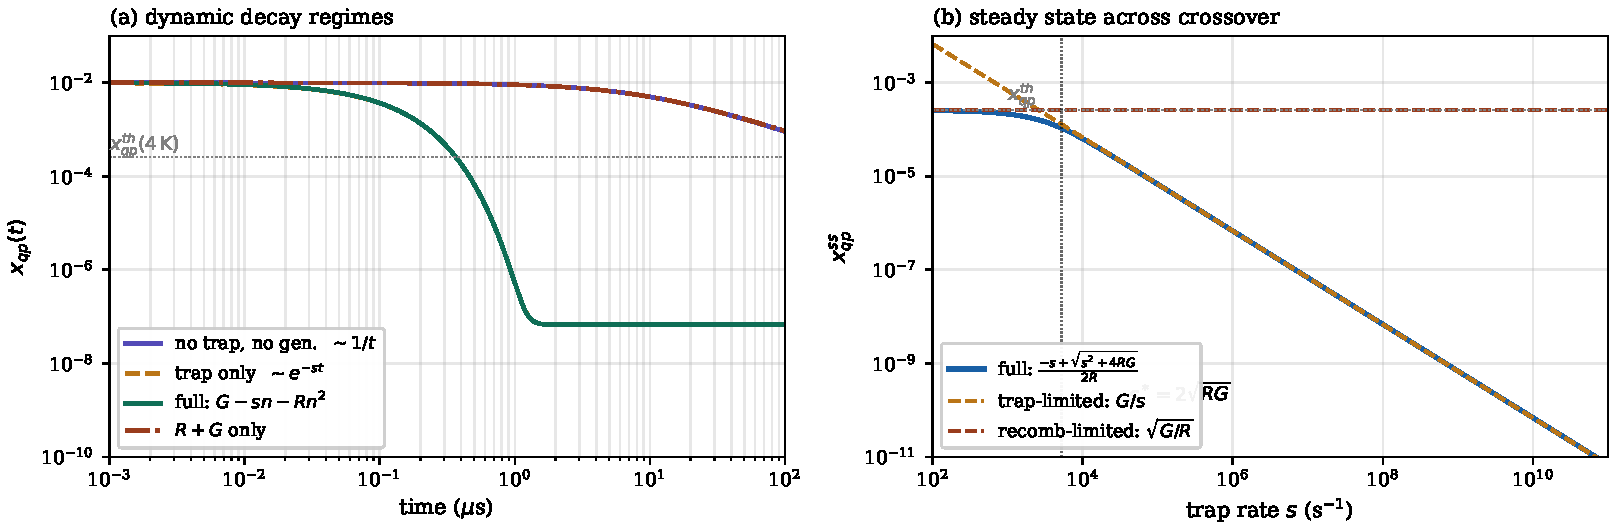
\includegraphics[width=\textwidth]{chapters/qh_figures/fig_kinetic_regimes.pdf}
  \caption{Analytical solutions of the reduced kinetic
    equation~\eqref{app:qp:eq:reduced-kinetic}, verified against numerical
    ODE integration. (a)~Dynamic decay from a pulse injection
    $n_0 = 10^{-2}$ for the three limiting cases. (b)~Steady-state
    density as a function of the trap rate $s$, showing the crossover at
    $s^* = 2\sqrt{R G}$ between recombination-limited ($\sqrt{G/R}$) and
    trap-limited ($G/s$) behaviour. Parameters: $R = 10^7\,{\rm s}^{-1}$
    (NbN benchmark), $G = R\,(\xqpth)^2$ at \SI{4}{\kelvin}.}
  \label{app:qp:fig:kinetic-regimes}
\end{figure}


\section{Implications for an NbN transmon at \SI{4}{\kelvin}}
\label{app:qp:implications}

The intrinsic quasiparticle-induced relaxation rate for a transmon is given,
in the small-$\hbar\omega/\Delta$ limit, by~\cite{Catelani2011}
\begin{equation}
  \frac{1}{T_1^{\rm qp}}
  \;=\; \frac{\omega_{01}}{\pi}\,\xqp\,
        \sqrt{\frac{2\Delta}{\hbar\omega_{01}}}\,.
  \label{app:qp:eq:T1qp}
\end{equation}
For NbN at \SI{4}{\kelvin}, with $\Delta = \SI{2.8}{\milli\electronvolt}$
and $\omega_{01}/2\pi = \SI{5}{\giga\hertz}$, substituting
$\xqp = \xqpth = 2.7\times 10^{-4}$ gives
\begin{equation}
  T_1^{\rm qp,\,intrinsic} \;\simeq\; \SI{20}{\nano\second}\,.
  \label{app:qp:eq:T1-intrinsic}
\end{equation}
Reaching a coherence time of $T_1 = \SI{49}{\micro\second}$, compatible with
the gate fidelities required by the algorithms discussed in
Chapter~\ref{chap:algorithms}, therefore requires reducing $\xqp$ below its
thermal-equilibrium value by approximately three orders of magnitude. Two
engineering approaches are conceivable: \emph{gap engineering}, which
exponentially suppresses one of the two tunneling channels across an
asymmetric junction, and \emph{trap engineering}, which lowers $\xqp$ in the
steady state of the kinetic balance. We examine both, and conclude that
only the latter is effective in the thermal regime.


\section{Why gap engineering does not work at \SI{4}{\kelvin}}
\label{app:qp:gap-fails}

In an asymmetric Josephson junction with electrode gaps $\Delta_1 > \Delta_2$,
Marchegiani \emph{et al.}~\cite{Marchegiani2022} have shown that quasiparticle
tunneling from the low-gap electrode is suppressed by a factor
$\exp[-(\Delta_1 - \Delta_2)/\kBb T]$ \emph{provided the quasiparticles are
out of thermal equilibrium}.  In that regime the population on the low-gap
side is fixed externally, and the suppression genuinely reduces the rate.
At \SI{4}{\kelvin}, however, both sides of the junction are in thermal
equilibrium with the phonon bath, and the population on the low-gap side
satisfies $\xqp^{\rm th}(\Delta_2) \gg \xqp^{\rm th}(\Delta_1)$.  The two
contributions to the total tunneling rate read
\begin{align}
  \Gamma_{1\to 2}
   &\;\propto\; \xqp^{\rm th}(\Delta_1)
   \qquad &&\text{(downhill, not suppressed)}\,,
   \label{app:qp:eq:rate-down}\\
  \Gamma_{2\to 1}
   &\;\propto\; \xqp^{\rm th}(\Delta_2)\,e^{-(\Delta_1-\Delta_2)/\kBb T}
   \qquad &&\text{(uphill, suppressed)}\,.
   \label{app:qp:eq:rate-up}
\end{align}
Substituting Eq.~\eqref{app:qp:eq:xqp-thermal}, the factor
$e^{-\Delta_2/\kBb T}$ in $\xqp^{\rm th}(\Delta_2)$ cancels against the
suppression $e^{-(\Delta_1-\Delta_2)/\kBb T}$, leaving
\begin{equation}
  \Gamma_{2\to 1}
   \;\propto\; \sqrt{\Delta_1/\Delta_2}\,\,\xqp^{\rm th}(\Delta_1)\,,
\end{equation}
of the same order as $\Gamma_{1\to 2}$.  The total rate is governed by
$e^{-\Delta_{\max}/\kBb T}$, i.e.\ by the larger gap, and is essentially
independent of the gap asymmetry.  Numerical evaluation with our kinetic
model confirms this: across the range of realistic candidate materials
(NbN/Nb, NbN/NbTiN, NbN/TaN), the $T_1^{\rm qp}$ at \SI{4}{\kelvin}
remains within a factor of two of the symmetric NbN/NbN baseline.
Gap engineering retains its value as a defence against cosmic-ray
quasiparticle bursts~\cite{McEwen2024} and for charge-parity
preservation~\cite{Kamenov2024}, but does not by itself relax the thermal
ceiling on $T_1^{\rm qp}$.


\section{Trap engineering: the working route}
\label{app:qp:traps}

A region of normal metal in tunnel contact with the superconductor provides
a sink for quasiparticles.  A quasiparticle that crosses the N--S barrier
relaxes inelastically to subgap energies in the normal metal, and the
superconducting gap then prevents its return
(Fig.~\ref{app:qp:fig:trap-mechanism}a).  In the diffusive regime, the
effective trap rate $s$ depends on the trap area $A_{\rm trap}$, on its
tunnel transparency $T_{\rm NS}$, on the normal-metal electron--electron
relaxation rate, and on the geometric configuration of the qubit pads:
the underlying spatial problem is one of diffusion to localised
sinks~\cite{Riwar2016,Hosseinkhani2017}.

\begin{figure}[t]
  \centering
  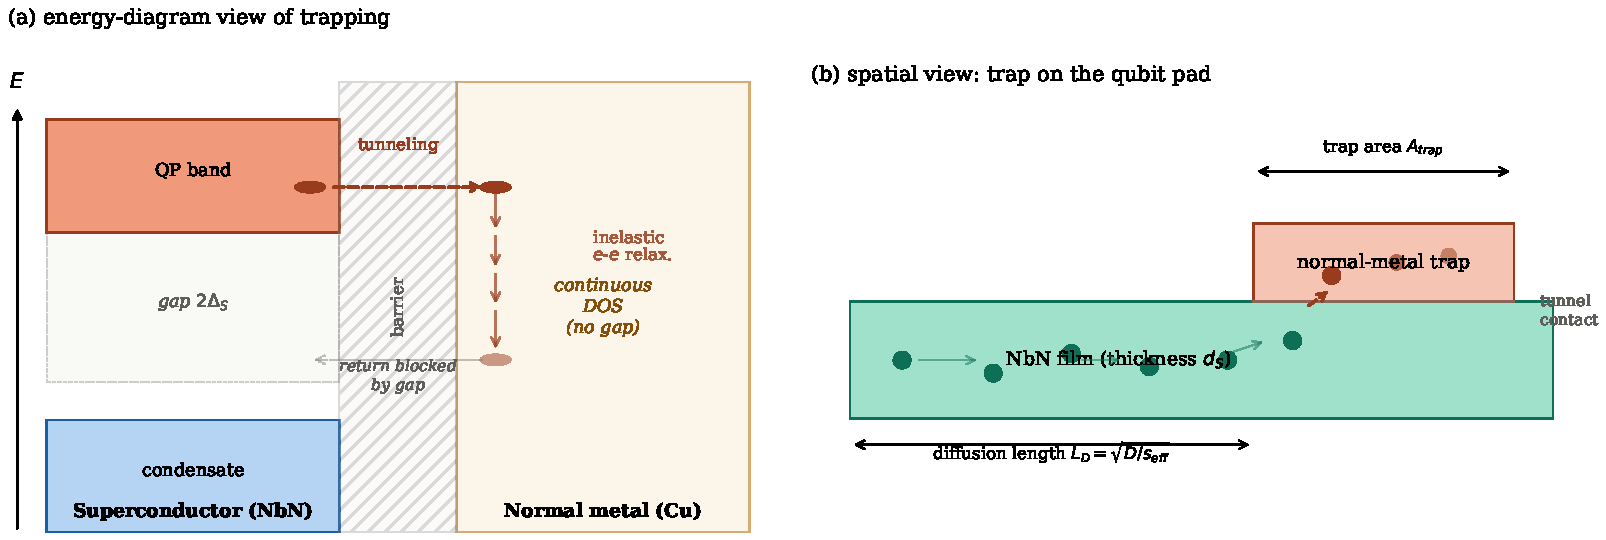
\includegraphics[width=\textwidth]{chapters/qh_figures/fig_trap_mechanism.pdf}
  \caption{Normal-metal trap mechanism.
    (a)~Energy diagram: a quasiparticle tunnels from the QP band of the
    superconductor into the continuous density of states of the normal
    metal, relaxes inelastically to subgap energies, and cannot return
    because the gap blocks the way.
    (b)~Spatial view: a quasiparticle diffusing in the NbN film with
    diffusion length $L_D = \sqrt{D/s_{\rm eff}}$ is captured by the
    normal-metal pad of area $A_{\rm trap}$ deposited in tunnel contact.}
  \label{app:qp:fig:trap-mechanism}
\end{figure}

Within Eq.~\eqref{app:qp:eq:nss-full} the requirement that
$\xqp^{\rm ss}$ falls sufficiently below the thermal floor to support
$T_1 = \SI{49}{\micro\second}$ can be expressed as a constraint on $s$.
Using Eq.~\eqref{app:qp:eq:T1qp} with the parameters of
Sec.~\ref{app:qp:implications}, the target reads
$\xqp \simeq 1.1\times 10^{-7}$.  In the trap-limited regime,
\begin{equation}
  s_{\rm min}
   \;=\; \frac{G_{\rm th}}{\xqp^{\rm target}}
   \;=\; \frac{R\,(\xqpth)^2}{\xqp^{\rm target}}
   \;\sim\; 10^{7}\,{\rm s}^{-1}\,.
  \label{app:qp:eq:s-min}
\end{equation}
This is approximately one order of magnitude above the rates demonstrated
in aluminum-based devices, where $s \sim 10^{4}$--$10^{6}$~s$^{-1}$ has
been measured~\cite{Riwar2016}. Reaching the target therefore requires
trap engineering at the upper edge of what has been experimentally
demonstrated, and constitutes the open experimental question discussed
below.

\subsection{Implementation strategy}
\label{app:qp:trap-implementation}

We propose deposition of normal-metal patches---of dimensions and material
detailed in Fig.~\ref{app:qp:fig:trap-engineering}---on the capacitor pads
of the asymmetric SQUID transmon, on both sides of the junctions
(\emph{bilateral} trap configuration).  The choice is dictated by the
analysis of Sec.~\ref{app:qp:gap-fails}: since the kinetic limit on $T_1$
is set by the sum of two tunneling channels, both of comparable magnitude
in thermal equilibrium, only suppressing $\xqp$ on \emph{both} electrodes
yields the multiplicative improvement.

The relevant design parameters are: the material of the trap
(Cu, Au, or Pd, with progressively shorter electron--electron relaxation
times), its area $A_{\rm trap}$, its thickness, and its distance $L$ from
the junction.  The effective trap rate in the diffusion-limited regime
saturates at $s_{\rm sat} \simeq D/L^2$, where $D$ is the quasiparticle
diffusion coefficient in NbN; pushing $s$ beyond $s_{\rm sat}$ is not
possible by increasing the trap area, and requires reducing $L$ or
increasing $D$ (cleaner films).

\begin{figure}[t]
  \centering
  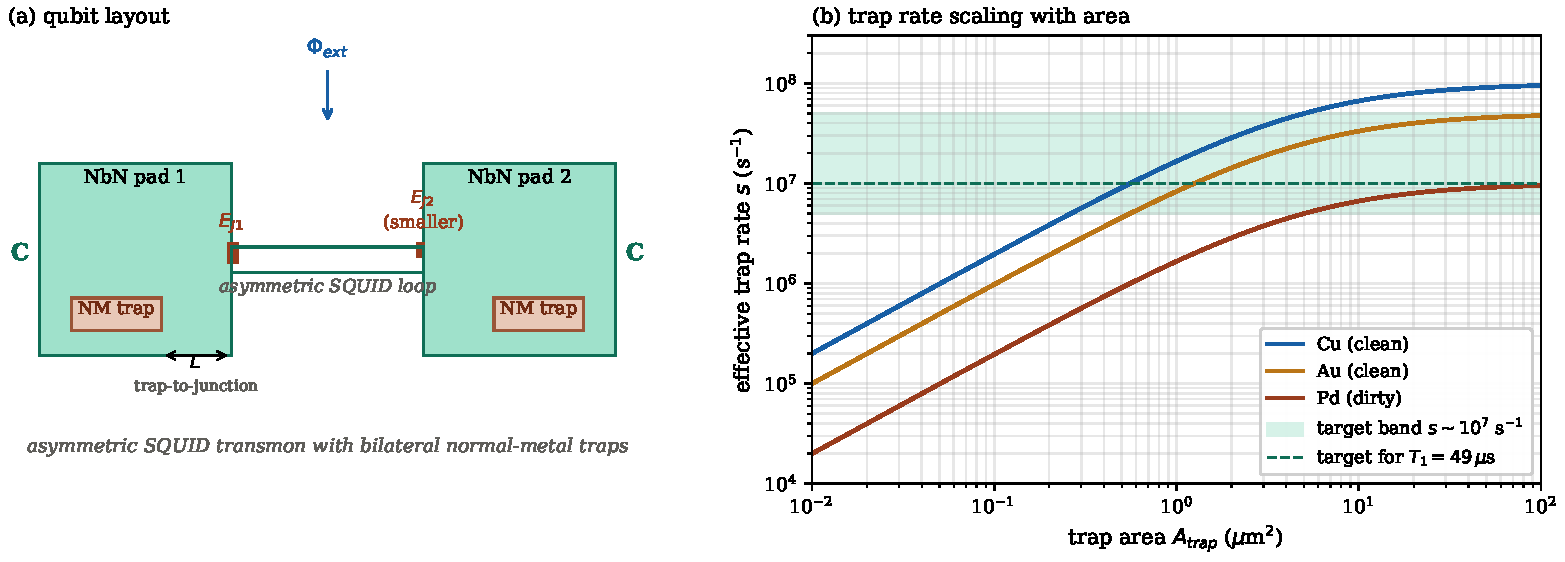
\includegraphics[width=\textwidth]{chapters/qh_figures/fig_trap_engineering.pdf}
  \caption{Trap engineering for the asymmetric SQUID transmon.
    (a)~Proposed device layout: normal-metal traps deposited on both NbN
    capacitor pads, at distance $L$ from the asymmetric SQUID. External
    flux $\Phi_{\rm ext}$ tunes the operating point between upper (USS,
    $\Phi=0$) and lower sweet spot (LSS, $\Phi=\Phi_0/2$), with the
    geometric junction asymmetry $d = (\Eone-\Etwo)/(\Eone+\Etwo)$ keeping
    $\omega_{01}$ finite at the LSS.
    (b)~Effective trap rate $s$ as a function of trap area
    $A_{\rm trap}$, for three candidate normal metals.  Saturation at
    large area reflects the diffusion-limited regime
    $s_{\rm sat} \simeq D/L^2$.  The target band $s \sim 10^{7}\,{\rm s}^{-1}$
    is required to reach $T_1 = \SI{49}{\micro\second}$ at
    \SI{4}{\kelvin}.}
  \label{app:qp:fig:trap-engineering}
\end{figure}

A trade-off exists between trap efficiency and microwave dissipation: the
normal-metal patch introduces a loss tangent that lowers the qubit quality
factor through capacitive coupling.  Locating the traps far enough from
the high-electric-field region near the junction (large $L$), while still
in the diffusion-reach of the quasiparticles, is therefore essential.
Quantitative estimation of the loss penalty requires electromagnetic
simulation of the participation ratio of the trap region, which is left
to follow-up work.


\section{Outlook}
\label{app:qp:outlook}

The analysis presented here identifies trap engineering as the only
quantitatively viable route to a microsecond-range $T_1$ in a NbN transmon
operated at \SI{4}{\kelvin}, the temperature accessible with a
two-stage pulse-tube cryocooler without sub-Kelvin refrigeration.  The
required trap rate $s \sim 10^{7}\,{\rm s}^{-1}$ sits approximately one
order of magnitude above the state of the art in aluminum-based devices
and has not been demonstrated in NbN.  The realisation of trap-engineered
NbN qubits at this performance level remains an open experimental
question, and constitutes a natural extension of the work presented in
this thesis.

%
% Cross-references defined here (so quantum_algorithms.tex can \cref them):
%   \label{app:qp}, \label{app:qp:kinetic}, \label{app:qp:traps},
%   \label{app:qp:eq:nss-full}, \label{app:qp:eq:s-min}
% ========================================================================

\chapter[Quasiparticle generation, population, and trapping]%
        {Quasiparticle generation, population, and trapping\\
         in superconducting transmons at \SI{4}{\kelvin}}
\label{app:qp}

% Custom commands - only define if not already in main preamble
\providecommand{\xqp}{x_{\rm qp}}
\providecommand{\xqpth}{x_{\rm qp}^{\rm th}}
\providecommand{\kBb}{k_{\rm B}}
\providecommand{\Eone}{E_{J1}}
\providecommand{\Etwo}{E_{J2}}

\section{Bogoliubov quasiparticles and Fermi--Dirac statistics}
\label{app:qp:bogoliubov}

The elementary excitations of a BCS superconductor are not Cooper pairs but
\emph{Bogoliubov quasiparticles}, coherent superpositions of an electron and a
hole created by
\begin{equation}
  \gamma^\dagger_{k\sigma}
   \;=\; u_k\, c^\dagger_{k\sigma} \;-\; \sigma v_k\, c_{-k,-\sigma}\,,
  \label{app:qp:eq:bogoliubov}
\end{equation}
with coherence factors satisfying $u_k^2 + v_k^2 = 1$.  The associated
dispersion is
\begin{equation}
  E_k \;=\; \sqrt{\xi_k^2 + \Delta^2}\,,\qquad E_k \geq \Delta\,,
  \label{app:qp:eq:bcs-dispersion}
\end{equation}
where $\xi_k$ is the normal-state energy measured from the Fermi level and
$\Delta$ is the superconducting gap.  Because these excitations inherit the
anticommutation relations of the underlying fermionic operators, they obey
Fermi--Dirac statistics rather than Bose--Einstein.  The phonons of the
crystal lattice are bosonic, but the dissipation channel that limits qubit
coherence---tunneling of single quasiparticles through the Josephson
junction---is purely fermionic.

This distinction has two practical consequences.  First, the excitation
spectrum is gapped: producing a quasiparticle costs at least $\Delta$, so the
thermal population is exponentially suppressed.  Second, the BCS density of
states diverges at the gap edge,
\begin{equation}
  N_S(E)
  \;=\; N(0)\,\frac{|E|}{\sqrt{E^2-\Delta^2}}\,,
  \qquad |E| \geq \Delta\,,
  \label{app:qp:eq:bcs-dos}
\end{equation}
amplifying the contribution of low-energy quasiparticles which dominate
tunneling. Both features are visible in
Fig.~\ref{app:qp:fig:generation-population}.


\section{Generation and thermal population}
\label{app:qp:generation}

A phonon with energy $\hbar\omega \geq 2\Delta$ breaks a Cooper pair and
generates two quasiparticles at the gap edge,
$\gamma_e\,(E=+\Delta)$ and $\gamma_h\,(E=-\Delta)$
(Fig.~\ref{app:qp:fig:generation-population}a).  Detailed balance with the
phonon bath fixes the equilibrium density.  Folding
Eq.~\eqref{app:qp:eq:bcs-dos} with the Fermi--Dirac distribution and
integrating, in the limit $\kBb T \ll \Delta$ one obtains
\begin{equation}
  \boxed{\;
    \xqpth(T)
    \;\equiv\; \frac{n_{\rm qp}}{n_{\rm cp}}
    \;\simeq\; \sqrt{\frac{2\pi \kBb T}{\Delta}}\,\exp\!\left(-\frac{\Delta}{\kBb T}\right)\,,
  \;}
  \label{app:qp:eq:xqp-thermal}
\end{equation}
where $n_{\rm cp} = 2N(0)\Delta$ is the Cooper-pair density.  For NbN at the
target operating temperature $T = \SI{4}{\kelvin}$, with
$\Delta \simeq \SI{2.8}{\milli\electronvolt}$, we obtain
$\xqpth(\SI{4}{\kelvin}) \simeq 2.7 \times 10^{-4}$.  This number is the
\emph{thermal floor}: any non-equilibrium contribution decreases the steady
state below this value only if a removal mechanism with rate exceeding the
phonon-driven generation is provided.

\begin{figure}[t]
  \centering
  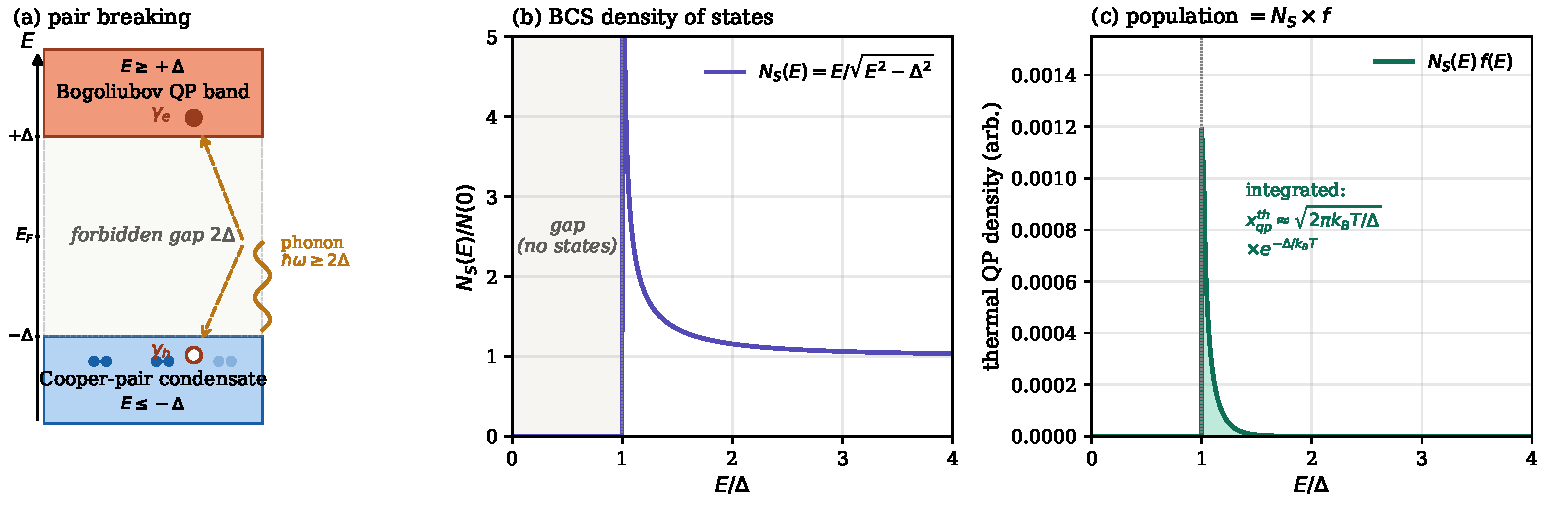
\includegraphics[width=\textwidth]{chapters/qh_figures/fig_qp_generation_population.pdf}
  \caption{Quasiparticle physics in three panels.
    (a)~A phonon with $\hbar\omega \geq 2\Delta$ breaks a Cooper pair,
    producing an electron-like quasiparticle $\gamma_e$ at $E=+\Delta$ and a
    hole-like quasiparticle $\gamma_h$ at $E=-\Delta$.
    (b)~The BCS density of states (Eq.~\ref{app:qp:eq:bcs-dos}) diverges at
    $|E| = \Delta$.
    (c)~The thermal population $N_S(E)\,f(E)$ is concentrated within a
    few $\kBb T$ of the gap edge; the integrated density is given by
    Eq.~\ref{app:qp:eq:xqp-thermal}.}
  \label{app:qp:fig:generation-population}
\end{figure}


\section{Kinetic equations: Rothwarf--Taylor with traps}
\label{app:qp:kinetic}

The dynamics of the integrated quasiparticle density $n$ and of the population
$N$ of pair-breaking phonons ($\hbar\omega = 2\Delta$) follow the
Rothwarf--Taylor equations~\cite{Rothwarf1967}, here augmented by an
empirical trap rate $s$ acting on quasiparticles:
\begin{align}
  \dot n &= I_{qp} \;+\; 2\beta N \;-\; R\,n^2 \;-\; s\,n\,,
  \label{app:qp:eq:RT-n}\\[2pt]
  \dot N &= I_{ph} \;-\; \beta N \;+\; \tfrac{1}{2} R\,n^2
            \;-\; \gamma_{\rm esc}\,(N - N_{\rm eq})\,.
  \label{app:qp:eq:RT-N}
\end{align}
$R$ is the bimolecular recombination coefficient
($R = 2/(n_{\rm cp}\,\tau_R^{\rm eq})$, with $\tau_R$ from
Kaplan~\cite{Kaplan1976}); $\beta$ the pair-breaking coefficient;
$\gamma_{\rm esc}$ the rate at which $2\Delta$ phonons escape to the
substrate; $I_{qp}, I_{ph}$ external sources.  Eliminating $N$ in the steady
state and defining the effective recombination rate
$R_{\rm eff} = R\,\gamma_{\rm esc}/(\beta + \gamma_{\rm esc})$, the
quasiparticle equation reduces to
\begin{equation}
  \dot n
  \;=\; G \;-\; s\,n \;-\; R_{\rm eff}\,n^2\,,
  \label{app:qp:eq:reduced-kinetic}
\end{equation}
with $G$ a total effective generation rate fixed by detailed balance
($G = R_{\rm eff}\,n_{\rm eq}^2$ in the absence of external sources).
Equation~\eqref{app:qp:eq:reduced-kinetic} is a Riccati equation and admits
closed-form analytical solutions in three regimes.

\subsection{Regime~1: pure relaxation, no generation, no trap}

For $G=s=0$ and initial condition $n(0)=n_0$, the equation
$\dot n = -R\,n^2$ separates and integrates to
\begin{equation}
  n(t) \;=\; \frac{n_0}{1 + R\,n_0\, t}\,.
  \label{app:qp:eq:hyperbolic-decay}
\end{equation}
The decay is \emph{hyperbolic}, not exponential. This is the signature of
bimolecular recombination: two quasiparticles are required to form a Cooper
pair, so the rate scales as $n^2$. This $1/t$ behaviour is observed in
pump-probe experiments on MgB$_2$ and Pb~\cite{Demsar2003}.

\subsection{Regime~2: trap-dominated linear decay}

When $s\,n \gg R\,n^2$ (sufficiently low density or sufficiently large $s$),
Eq.~\eqref{app:qp:eq:reduced-kinetic} linearises to $\dot n = G - s\,n$,
yielding
\begin{equation}
  n(t) \;=\; n^{\rm ss} \;+\; (n_0 - n^{\rm ss})\,e^{-s\,t}\,,
  \qquad n^{\rm ss} \;=\; \frac{G}{s}\,.
  \label{app:qp:eq:trap-linear}
\end{equation}
The decay is exponential, with time constant $\tau_{\rm tr} = 1/s$. This is
the regime in which normal-metal traps operate in transmon
qubits~\cite{Riwar2016}.

\subsection{Regime~3: full Riccati solution}

The general steady-state solution is obtained from the positive root of
$G - s n - R n^2 = 0$:
\begin{equation}
  \boxed{\;
    n^{\rm ss}
    \;=\; \frac{-\,s \;+\; \sqrt{s^2 + 4 R G}}{2 R}\,.
  \;}
  \label{app:qp:eq:nss-full}
\end{equation}
The crossover between the recombination-dominated and the trap-dominated
regime occurs at $s^* = 2\sqrt{R G}$: for $s \ll s^*$,
Eq.~\eqref{app:qp:eq:nss-full} reduces to $\sqrt{G/R}$
(recombination-limited); for $s \gg s^*$ it reduces to $G/s$
(trap-limited). The full time-dependent solution can be written in closed
form by separating variables; the relaxation rate towards the steady state
is $\Gamma_{\rm relax} = \sqrt{s^2 + 4 R G}$. The three regimes are
summarised in Fig.~\ref{app:qp:fig:kinetic-regimes} and compared with
direct numerical integration of Eq.~\eqref{app:qp:eq:reduced-kinetic}.

\begin{figure}[t]
  \centering
  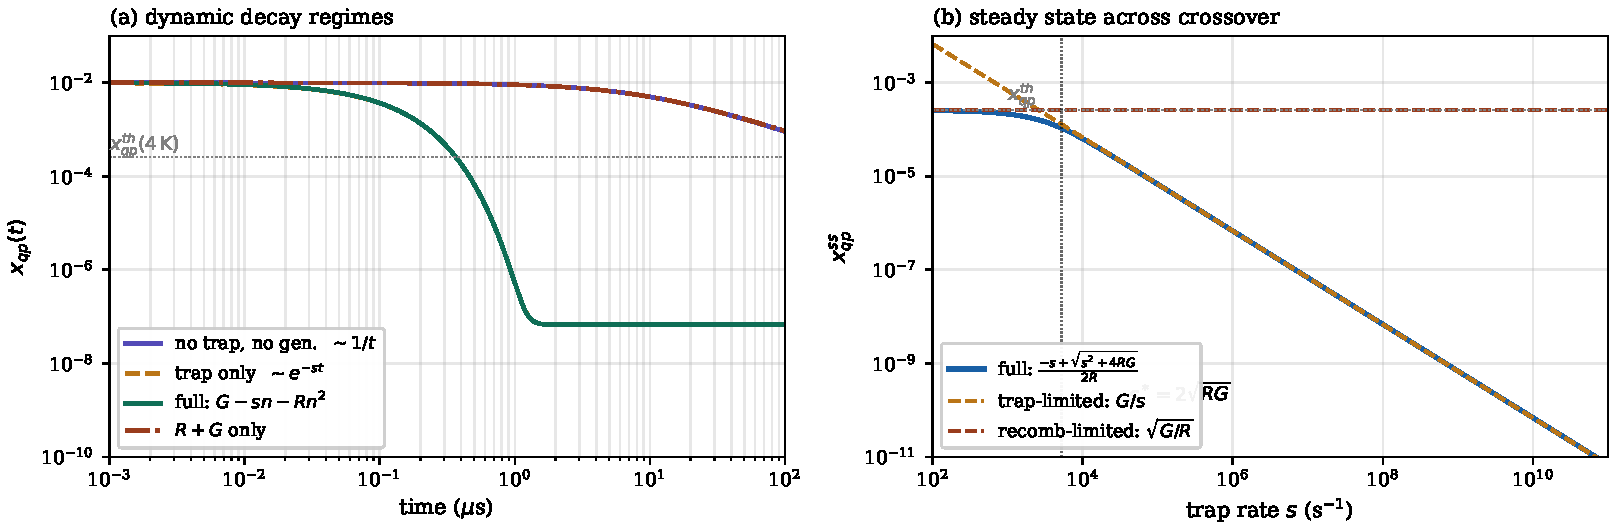
\includegraphics[width=\textwidth]{chapters/qh_figures/fig_kinetic_regimes.pdf}
  \caption{Analytical solutions of the reduced kinetic
    equation~\eqref{app:qp:eq:reduced-kinetic}, verified against numerical
    ODE integration. (a)~Dynamic decay from a pulse injection
    $n_0 = 10^{-2}$ for the three limiting cases. (b)~Steady-state
    density as a function of the trap rate $s$, showing the crossover at
    $s^* = 2\sqrt{R G}$ between recombination-limited ($\sqrt{G/R}$) and
    trap-limited ($G/s$) behaviour. Parameters: $R = 10^7\,{\rm s}^{-1}$
    (NbN benchmark), $G = R\,(\xqpth)^2$ at \SI{4}{\kelvin}.}
  \label{app:qp:fig:kinetic-regimes}
\end{figure}


\section{Implications for an NbN transmon at \SI{4}{\kelvin}}
\label{app:qp:implications}

The intrinsic quasiparticle-induced relaxation rate for a transmon is given,
in the small-$\hbar\omega/\Delta$ limit, by~\cite{Catelani2011}
\begin{equation}
  \frac{1}{T_1^{\rm qp}}
  \;=\; \frac{\omega_{01}}{\pi}\,\xqp\,
        \sqrt{\frac{2\Delta}{\hbar\omega_{01}}}\,.
  \label{app:qp:eq:T1qp}
\end{equation}
For NbN at \SI{4}{\kelvin}, with $\Delta = \SI{2.8}{\milli\electronvolt}$
and $\omega_{01}/2\pi = \SI{5}{\giga\hertz}$, substituting
$\xqp = \xqpth = 2.7\times 10^{-4}$ gives
\begin{equation}
  T_1^{\rm qp,\,intrinsic} \;\simeq\; \SI{20}{\nano\second}\,.
  \label{app:qp:eq:T1-intrinsic}
\end{equation}
Reaching a coherence time of $T_1 = \SI{49}{\micro\second}$, compatible with
the gate fidelities required by the algorithms discussed in
Chapter~\ref{chap:algorithms}, therefore requires reducing $\xqp$ below its
thermal-equilibrium value by approximately three orders of magnitude. Two
engineering approaches are conceivable: \emph{gap engineering}, which
exponentially suppresses one of the two tunneling channels across an
asymmetric junction, and \emph{trap engineering}, which lowers $\xqp$ in the
steady state of the kinetic balance. We examine both, and conclude that
only the latter is effective in the thermal regime.


\section{Why gap engineering does not work at \SI{4}{\kelvin}}
\label{app:qp:gap-fails}

In an asymmetric Josephson junction with electrode gaps $\Delta_1 > \Delta_2$,
Marchegiani \emph{et al.}~\cite{Marchegiani2022} have shown that quasiparticle
tunneling from the low-gap electrode is suppressed by a factor
$\exp[-(\Delta_1 - \Delta_2)/\kBb T]$ \emph{provided the quasiparticles are
out of thermal equilibrium}.  In that regime the population on the low-gap
side is fixed externally, and the suppression genuinely reduces the rate.
At \SI{4}{\kelvin}, however, both sides of the junction are in thermal
equilibrium with the phonon bath, and the population on the low-gap side
satisfies $\xqp^{\rm th}(\Delta_2) \gg \xqp^{\rm th}(\Delta_1)$.  The two
contributions to the total tunneling rate read
\begin{align}
  \Gamma_{1\to 2}
   &\;\propto\; \xqp^{\rm th}(\Delta_1)
   \qquad &&\text{(downhill, not suppressed)}\,,
   \label{app:qp:eq:rate-down}\\
  \Gamma_{2\to 1}
   &\;\propto\; \xqp^{\rm th}(\Delta_2)\,e^{-(\Delta_1-\Delta_2)/\kBb T}
   \qquad &&\text{(uphill, suppressed)}\,.
   \label{app:qp:eq:rate-up}
\end{align}
Substituting Eq.~\eqref{app:qp:eq:xqp-thermal}, the factor
$e^{-\Delta_2/\kBb T}$ in $\xqp^{\rm th}(\Delta_2)$ cancels against the
suppression $e^{-(\Delta_1-\Delta_2)/\kBb T}$, leaving
\begin{equation}
  \Gamma_{2\to 1}
   \;\propto\; \sqrt{\Delta_1/\Delta_2}\,\,\xqp^{\rm th}(\Delta_1)\,,
\end{equation}
of the same order as $\Gamma_{1\to 2}$.  The total rate is governed by
$e^{-\Delta_{\max}/\kBb T}$, i.e.\ by the larger gap, and is essentially
independent of the gap asymmetry.  Numerical evaluation with our kinetic
model confirms this: across the range of realistic candidate materials
(NbN/Nb, NbN/NbTiN, NbN/TaN), the $T_1^{\rm qp}$ at \SI{4}{\kelvin}
remains within a factor of two of the symmetric NbN/NbN baseline.
Gap engineering retains its value as a defence against cosmic-ray
quasiparticle bursts~\cite{McEwen2024} and for charge-parity
preservation~\cite{Kamenov2024}, but does not by itself relax the thermal
ceiling on $T_1^{\rm qp}$.


\section{Trap engineering: the working route}
\label{app:qp:traps}

A region of normal metal in tunnel contact with the superconductor provides
a sink for quasiparticles.  A quasiparticle that crosses the N--S barrier
relaxes inelastically to subgap energies in the normal metal, and the
superconducting gap then prevents its return
(Fig.~\ref{app:qp:fig:trap-mechanism}a).  In the diffusive regime, the
effective trap rate $s$ depends on the trap area $A_{\rm trap}$, on its
tunnel transparency $T_{\rm NS}$, on the normal-metal electron--electron
relaxation rate, and on the geometric configuration of the qubit pads:
the underlying spatial problem is one of diffusion to localised
sinks~\cite{Riwar2016,Hosseinkhani2017}.

\begin{figure}[t]
  \centering
  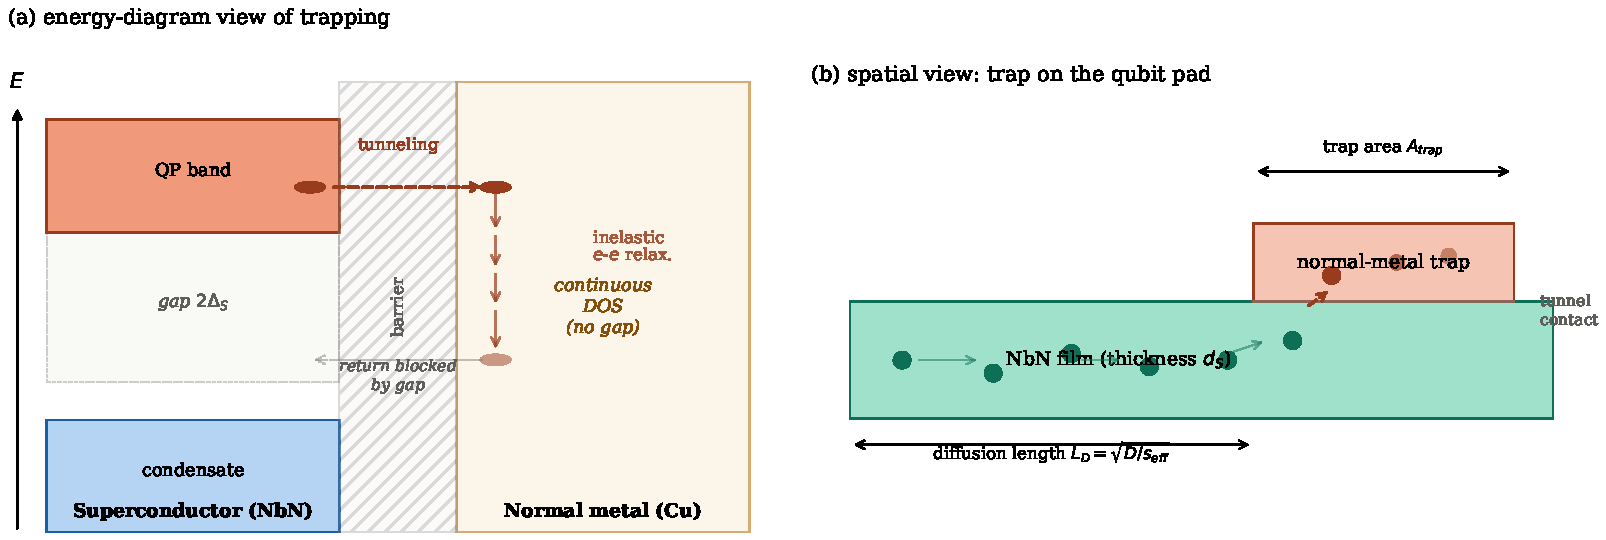
\includegraphics[width=\textwidth]{chapters/qh_figures/fig_trap_mechanism.pdf}
  \caption{Normal-metal trap mechanism.
    (a)~Energy diagram: a quasiparticle tunnels from the QP band of the
    superconductor into the continuous density of states of the normal
    metal, relaxes inelastically to subgap energies, and cannot return
    because the gap blocks the way.
    (b)~Spatial view: a quasiparticle diffusing in the NbN film with
    diffusion length $L_D = \sqrt{D/s_{\rm eff}}$ is captured by the
    normal-metal pad of area $A_{\rm trap}$ deposited in tunnel contact.}
  \label{app:qp:fig:trap-mechanism}
\end{figure}

Within Eq.~\eqref{app:qp:eq:nss-full} the requirement that
$\xqp^{\rm ss}$ falls sufficiently below the thermal floor to support
$T_1 = \SI{49}{\micro\second}$ can be expressed as a constraint on $s$.
Using Eq.~\eqref{app:qp:eq:T1qp} with the parameters of
Sec.~\ref{app:qp:implications}, the target reads
$\xqp \simeq 1.1\times 10^{-7}$.  In the trap-limited regime,
\begin{equation}
  s_{\rm min}
   \;=\; \frac{G_{\rm th}}{\xqp^{\rm target}}
   \;=\; \frac{R\,(\xqpth)^2}{\xqp^{\rm target}}
   \;\sim\; 10^{7}\,{\rm s}^{-1}\,.
  \label{app:qp:eq:s-min}
\end{equation}
This is approximately one order of magnitude above the rates demonstrated
in aluminum-based devices, where $s \sim 10^{4}$--$10^{6}$~s$^{-1}$ has
been measured~\cite{Riwar2016}. Reaching the target therefore requires
trap engineering at the upper edge of what has been experimentally
demonstrated, and constitutes the open experimental question discussed
below.

\subsection{Implementation strategy}
\label{app:qp:trap-implementation}

We propose deposition of normal-metal patches---of dimensions and material
detailed in Fig.~\ref{app:qp:fig:trap-engineering}---on the capacitor pads
of the asymmetric SQUID transmon, on both sides of the junctions
(\emph{bilateral} trap configuration).  The choice is dictated by the
analysis of Sec.~\ref{app:qp:gap-fails}: since the kinetic limit on $T_1$
is set by the sum of two tunneling channels, both of comparable magnitude
in thermal equilibrium, only suppressing $\xqp$ on \emph{both} electrodes
yields the multiplicative improvement.

The relevant design parameters are: the material of the trap
(Cu, Au, or Pd, with progressively shorter electron--electron relaxation
times), its area $A_{\rm trap}$, its thickness, and its distance $L$ from
the junction.  The effective trap rate in the diffusion-limited regime
saturates at $s_{\rm sat} \simeq D/L^2$, where $D$ is the quasiparticle
diffusion coefficient in NbN; pushing $s$ beyond $s_{\rm sat}$ is not
possible by increasing the trap area, and requires reducing $L$ or
increasing $D$ (cleaner films).

\begin{figure}[t]
  \centering
  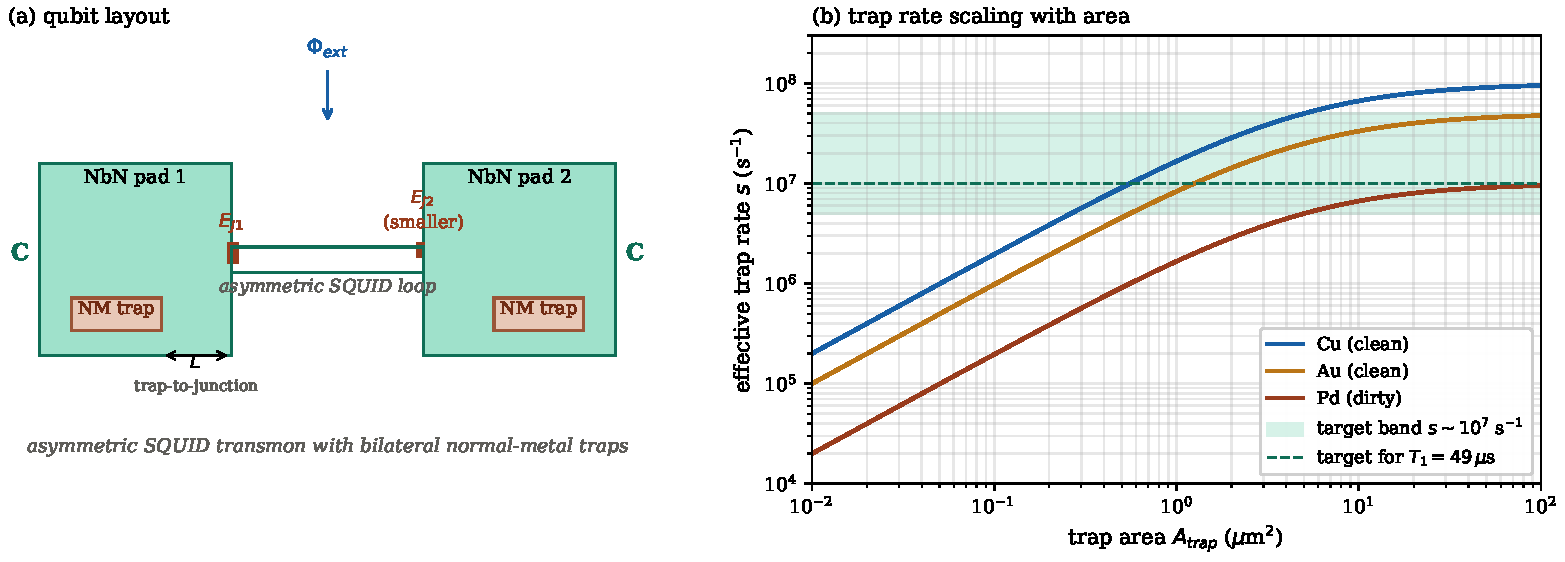
\includegraphics[width=\textwidth]{chapters/qh_figures/fig_trap_engineering.pdf}
  \caption{Trap engineering for the asymmetric SQUID transmon.
    (a)~Proposed device layout: normal-metal traps deposited on both NbN
    capacitor pads, at distance $L$ from the asymmetric SQUID. External
    flux $\Phi_{\rm ext}$ tunes the operating point between upper (USS,
    $\Phi=0$) and lower sweet spot (LSS, $\Phi=\Phi_0/2$), with the
    geometric junction asymmetry $d = (\Eone-\Etwo)/(\Eone+\Etwo)$ keeping
    $\omega_{01}$ finite at the LSS.
    (b)~Effective trap rate $s$ as a function of trap area
    $A_{\rm trap}$, for three candidate normal metals.  Saturation at
    large area reflects the diffusion-limited regime
    $s_{\rm sat} \simeq D/L^2$.  The target band $s \sim 10^{7}\,{\rm s}^{-1}$
    is required to reach $T_1 = \SI{49}{\micro\second}$ at
    \SI{4}{\kelvin}.}
  \label{app:qp:fig:trap-engineering}
\end{figure}

A trade-off exists between trap efficiency and microwave dissipation: the
normal-metal patch introduces a loss tangent that lowers the qubit quality
factor through capacitive coupling.  Locating the traps far enough from
the high-electric-field region near the junction (large $L$), while still
in the diffusion-reach of the quasiparticles, is therefore essential.
Quantitative estimation of the loss penalty requires electromagnetic
simulation of the participation ratio of the trap region, which is left
to follow-up work.


\section{Outlook}
\label{app:qp:outlook}

The analysis presented here identifies trap engineering as the only
quantitatively viable route to a microsecond-range $T_1$ in a NbN transmon
operated at \SI{4}{\kelvin}, the temperature accessible with a
two-stage pulse-tube cryocooler without sub-Kelvin refrigeration.  The
required trap rate $s \sim 10^{7}\,{\rm s}^{-1}$ sits approximately one
order of magnitude above the state of the art in aluminum-based devices
and has not been demonstrated in NbN.  The realisation of trap-engineered
NbN qubits at this performance level remains an open experimental
question, and constitutes a natural extension of the work presented in
this thesis.
